\chapter{Automated Sparse Tiling for Irregular Computations}
\label{ch:sparsetiling}

Many numerical methods for partial differential equations (PDEs) are structured as sequences of parallel loops. This exposes parallelism well, but does not convert data reuse between loops into data locality, since their working set is usually too big to fit in some level of cache. In Section~\ref{sec:bkg:poly}, it was explained that loop fusion and loop tiling may be used to retain some of this potential data locality. This chapter introduces a mixed compiler/library system capable of applying these transformations to sequences of irregular loops, automatically. Challenges deriving from real-world applications are addressed. As reiterated throughout the chapter, parts of this work are the result of a joint collaboration with~\cite{st-paper}.

\section{Motivation}
\label{sec:tiling:motivation}

The focus of this chapter is improving data locality in unstructured mesh PDE solvers, such as those based on the finite volume or the finite element methods. Here, the loop-to-loop dependence structure is data-dependent due to indirect references such as \texttt{A[map[i]]}. The \texttt{map} array stores connectivity information, for example from elements in the mesh to degrees of freedom. A similar pattern occurs in molecular dynamics simulations and graph processing, so both the theory and the tools that we will develop in this chapter are generalizable to these domains. 

Three motivating real-world applications for this work are Hydra, Volna and Seigen. Hydra~\citep{hydra-op2} is a computational fluid dynamics application used at Rolls Royce for the simulation of next-generation components of jet engines. Volna~\citep{ST-volna} is a computational fluid dynamics application for the modelling of tsunami waves. Seigen aims to solve the elastic wave equation using the discontinuous Galerkin finite element method for energy exploration purposes. All these applications are characterized by the presence of a time-stepping loop, in which several loops over the computational mesh (33 in Hydra, 10 in Volna, 28 in Seigen) are executed. These loops are characterized by the aforementioned irregular loop-to-loop dependence structure. We will use Seigen, as well as other simpler benchmarks, for performance evaluation.

Because of the irregular memory access pattern, our approach to loop transformation is based on dynamic analysis, particularly on \textit{inspector/executor schemes}. Among the possible dynamic loop optimizations, we target \textit{sparse tiling}. We recall from Section~\ref{sec:bkg:tiling} that sparse tiling aims to exploit data reuse across consecutive loops by composing two transformations, namely loop fusion and loop tiling. Given the presence of significant data reuse across consecutive loops, our hypothesis is that sparse tiling has potential in the class of unstructured mesh PDE solvers that we are targeting.

Summarizing, three main issues are tackled in this chapter:

\begin{itemize}
\item Previous approaches to sparse tiling were all based upon ``ad-hoc'' inspector/executor strategies; that is, developed ``by hand'', per application. We seek a general technique, applicable to arbitrary computations on unstructured meshes.
\item Automation is more than a desired feature because application specialists avoid complex optimizations harming source code comprehensibility. We therefore aim for a fully-automated framework, based upon domain-specific languages and a mixed compiler/library approach.
\item A few studies have addressed the problem of fusing loops when these need be interleaved by routines for message passing. However, we are aware of none for the scenario in which the memory accesses pattern is irregular. We fill this gap by introducing a sparse tiling scheme that performs redundant computation over partition boundaries to delay communication. The importance of this contribution stems from the fact that most scientific simulations require distributed-memory parallelism.
\end{itemize}

\section{Context and Approach}
\label{sec:tiling:struct}
Loop fusion and loop tiling have been widely studied in the literature. A considerable number of techniques for improving and automating these transformations have been proposed over the years. Their evaluation, however, has traditionally been limited to a small set of benchmarks (or ``mini-applications'') and single-node performance. In particular, it has repeatedly been shown that simple stencil codes arising in finite difference methods~\citep{vect-tiled-ho-fd,ics-stencil-tiling,cohen-timetiling}, linear algebra routines~\citep{qr-fact-tiled,blas-tiling}, and image processing kernels~\citep{Halide} can benefit from both loop fusion and loop tiling. This, unfortunately, does not shed light on the impact that these transformations could have in real-world applications, where the loop nests are often deeper, less structured, and characterized by irregular control flow. Since numerical methods for PDEs are often structured as sequences of complex, irregular loops (or ``sweeps'') over the computational mesh, some obvious questions arise: 

\begin{description}
\item[Applicability] Can sparse tiling be adopted in real-life numerical methods for solving PDEs, and should performance improvements be expected?
\item[Lack of evidence] Why, despite decades of research, non-trivial loop transformations are rarely used in scientific simulations? 
\item[Challenges] What are the theoretical and technical challenges that need be overcome to automate sparse tiling?
\end{description}

In this chapter, we tackle these problems in the following context:
\begin{description}
\item[Irregular codes] Unstructured meshes are often used to discretize the computational domain, since they allow for an accurate representation of complex geometries. Their connectivity is stored by means of adjacency lists (or equivalent data structure). This leads to indirect memory accesses within loop nests. Indirections break static analysis, thus making many compiler-based approaches to loop transformation (e.g., polyhedral optimization) ineffective. Runtime data dependence analysis enables dynamic loop optimization, although this results in additional overhead.
\item[Realistic datasets] Complex simulations usually operate on at least terabytes of data, hence execution on multi-node systems is required. Sparse tiling will have to coexist with distributed-memory parallelism.
\item[Automation, but no legacy code] Sparse tiling is an ``extreme optimization''. An implementation in a low level language (e.g., C, Fortran) requires a great deal of effort, as a thoughtful restructuring of the application is necessary. Similarly to many other low level transformations, it also makes the source code impenetrable, thus affecting maintenance and extendibility. We therefore aim for a fully automated system based on domain-specific languages, which abstracts sparse tiling through a simple interface (i.e., a single construct to tell the compiler ``transform the following sequence of loops'' ) and a tiny set of parameters for performance tuning (e.g., the tile size). We are not interested in supporting legacy code, where the key computational aspects (e.g., mesh iteration, distributed-memory parallelism) are usually hidden for software modularity, which makes automation almost impossible.
\end{description}

In this chapter, the problem of automatically applying sparse tiling to irregular codes based on shared- and distributed-memory parallelism is decomposed into two tasks:
\begin{enumerate}
\item establishing abstractions and devising algorithms to enable sparse tiling in arbitrary sequences of irregular loops (Sections~\ref{sec:tiling:lc}-\ref{sec:tiling:algo});
\item integration with a framework relying on domain-specific languages (Section~\ref{sec:tiling:automation}).
\end{enumerate}
Before addressing these two tasks, we elaborate on the theoretical and technical challenges that arise when applying loop fusion and loop tiling to real-world applications (Section~\ref{sec:tiling:difficult}), and review the related work (Section~\ref{sec:tiling:relatedwork}).  

%Finally, to summarize, our hypotheses are:
%\begin{itemize}
%\item Many loop nests in unstructured mesh applications are memory-bound, so exploiting the data reuse across consecutive loop nests should improve the performance.
%\item Applying sparse tiling is extremely complicated, so automation is necessary. However, automation presents challenges that none of the existing technologies can overcome. \end{itemize}

% Is skewing used for optimizing cross-time dependency, i.e., is the wave due to time?

\section{Applying Loop Fusion and Loop Tiling is More Difficult than Commonly Assumed}
\label{sec:tiling:difficult}
We show in Listing~\ref{code:tiling-struct} the ``skeleton'' of a typical PDE solver on an unstructured mesh. This will be useful throughout the analysis presented in this section.

\begin{algorithm}[t]
\scriptsize\ttfamily
\SetAlgorithmName{LISTING}{}

// Time-stepping loop (T = total number of iterations)\\
\KwSty{for} t = 1 \KwSty{to} T $\lbrace$\\
~~// 1st sweep over the $C$ cells of the mesh\\
~~\KwSty{for} i \KwSty{in} $C$ $\lbrace$\\
~~~~buffer$\_$0 = $\lbrace 0.0 \rbrace$  // will store the kernel output\\
~~~~buffer$\_$1 = gather$\_$data ( A[f(map[i])], ... )\\
~~~~...\\
~~~~kernel$\_$1( buffer$\_$0, buffer$\_$1, ... );\\
~~~~scatter$\_$data ( buffer$\_$0, f(map[i]) )\\
~~$\rbrace$\\
~~Calc (...);\\
~~MPI$\_$Comm (...); \\
~~// 2nd sweep over the $N$ nodes of the mesh\\
~~\KwSty{for} i \KwSty{in} $N$ $\lbrace$\\
~~~~... // Similar to sweep 1 \\
~~$\rbrace$\\
~~// Boundary conditions: sweep over the $BV$ boundary nodes\\
~~\KwSty{for} i \KwSty{in} $BV$ $\lbrace$\\
~~~~... // Similar to sweep 1 \\
~~$\rbrace$\\
~~...\\
~~Calc (...);\\
~~MPI$\_$Comm (...); \\
~~...\\
$\rbrace$
\caption{The ``bare'' structure of a numerical method for solving a PDE. Three parallelizable sweeps over the mesh -- in particular, over cells, nodes, and boundary nodes -- are executed within a time-stepping loop. In the cells loop, the invocation of a kernel is shown. First, the memory indirections are resolved and data is moved into suitable buffers. The data passed to the kernel is now contiguous in memory, which hopefully maximizes the chances of vectorization. Once the kernel has been executed, the computed values are ``scattered'' back from a buffer to memory. Distributed-memory parallelism is achieved through MPI, in particular through the {\tt MPI$\_$Comm (...)} calls that separate different mesh sweeps. Additional calculations, for instance in {\tt Calc (...)}, could also interleave the execution of consecutive loops.}
\label{code:tiling-struct}
\end{algorithm}

We identify three classes of problems that are often neglected, or at least treated with scarce emphasis, in the relevant literature. 

\begin{description}
\item[Theoretical questions] We first wonder about the effectiveness of loop fusion and loop tiling in unstructured mesh applications.

\begin{description}
\item[Computational boundedness] Computational methods for PDEs are structured as sequences of loop nests, each loop nest characterized by its own operational intensity. Within the same application, some loop nests may be memory-bound, while others CPU-bound. This clearly depends on the numerical method itself, particularly on aspects such as the arithmetic complexity of the operators and the type of discretization employed (e.g., polynomial order of function spaces). Obviously, if most loop nests are CPU-bound, the benefits of sparse tiling on data locality will provide marginal gains. Before even thinking about aggressive optimizations, it is fundamental to determine the bottlenecks of an application. This boils down to answering two questions: (i) what fraction of the execution time is due to memory-bound loop nests; (ii) can CPU-boundedness be relieved by applying other optimizations (e.g., vectorization).
\item[Loop tiling vs space filling curves] Loop tiling and space filling curves (SFCs) are two different attempts to solving the same problem: improving the performance of mesh-based computations by increasing data locality. SFCs provide an effective way of iterating over a mesh by guaranteeing that consecutive iterations correspond to neighboring elements; if these elements share some data values, data reuse is exploited. Just like loop tiling, SFCs can be considered loop reordering transformations (see Section~\ref{sec:bkg:loop-transf}). Unfortunately, the relationship between loop tiling and SFCs is unclear in the context of unstructured meshes. In this chapter, sparse tiling will be applied on top of SFCs.
\end{description}

\item[Technical issues] Recent works on fusion and tiling for structured mesh applications have addressed automation (e.g., polyhedral compilers), composition of transformations (e.g., time tiling), techniques for minimizing communication (e.g., diamond tiling). However, the following aspects were rarely given the attention they actually deserve.
\begin{description}
\item[Unstructured meshes] Although ad-hoc inspector-executor strategies for some proxy applications had previously been developed, general techniques for arbitrary computations on unstructured meshes have been missing until this thesis\footnote{We reinforce once more that the generalized sparse tiling algorithm is the result of a joint collaboration amongst the authors of~\citep{st-paper}.}. As already explained, the main problem with unstructured meshes is the presence of indirect memory accesses, which complicates the data dependence analysis needed for applying loop transformations.
\item[Time tiling and distributed-memory parallelism] We reiterate the fact that real-world computations require large-scale distributed-memory architectures. As Listing~\ref{code:tiling-struct} shows, MPI calls usually separate consecutive mesh sweeps. This poses a big challenge to time tiling, because now all tiles close to the boundary of a mesh partition require special handling.
\item[Time tiling and extra code] The {\tt Comp(...)} function in Listing~\ref{code:tiling-struct} shows that additional computation may be performed between consecutive mesh sweeps. {\tt Comp} could represent, for instance, check-pointing, I/O, or the resolution of a linear system through a function call to an external library. Moreover, conditional execution of loops (e.g., through \texttt{if-then-else}) may be present. The presence of additional code between loops make loop fusion extremely challenging. 
\item[Legacy code is usually impenetrable] Loop transformation opportunities are often hidden in existing scientific codes. As explained in~\cite{strout-common-problems}, common problems are: 1) potentially fusible or tilable loop nests are separated for code modularity; 2) handling of boundary conditions; 3) source code not amenable for data dependency analysis (e.g., extensive use of pointers, function calls).
\end{description}

\item[Limitations inherent in the numerical method] Two loops cannot be fused if they are separated by a global synchronization point. This is often a global reduction, either explicit (e.g., the first loop updates a global variable that is read by the second loop) or implicit (i.e., within an external function invoked between the two loops, like in many iterative solvers for linear systems). By limiting the applicability of many loop optimizations, global synchronization points pose great challenges and research questions. If strong scaling is the primary goal and memory-boundedness is the key limiting factor, then interesting questions are: (i) can the numerical method be reformulated to relieve the constraints on low level optimization (which requires a joint effort between application and performance specialists); (ii) can the tools be made more sophisticated to work around these problems; (iii) will the effort be rewarded by significant performance improvements.
\end{description}

All these issues will be addressed in the upcoming sections.

\section{Related Work}
\label{sec:tiling:relatedwork}

\subsection*{Loop Chain}
% Loop chain
The data dependence analysis that we develop in this chapter is based on an abstraction called \textit{loop chain}, which was originally presented in~\cite{ST-KriegerHIPS2013}. This abstraction is sufficiently general to capture data dependencies in programs structured as arbitrary sequences of loops. We will detail the loop chain abstraction in Section~\ref{sec:tiling:lc}.

\subsection*{Inspector/Executor and Sparse Tiling}
% Inspector/Executor
The loop chain abstraction provides sufficient information to create an inspector/executor scheme for an arbitrary unstructured mesh application. Inspector/executor strategies were first formalized by~\cite{ST-Saltz91}. They have been used exploiting data reuse and exposing shared-memory parallelism in several studies~\citep{ST-dimeEtna00,ST-StroutLCPC2002,ST-Demmel08,ST-KriegerIAAA2012}. 

Sparse tiling, which we introduced in Section~\ref{sec:bkg:ie}, is a technique based upon inspection/execution. The term was coined by~\cite{ST-StroutLCPC2002,ST-StroutIJHPCA} in the context of the Gauss-Seidel algorithm and in~\cite{ST-StroutPLDI03} in the context of the moldyn benchmark. However, the technique was initially proposed by~\cite{ST-dimeEtna00} to parallelize computations over unstructured meshes, taking the name of \textit{unstructured cache blocking}. In this work, the mesh was initially partitioned; the partitioning represented the tiling in the first sweep over the mesh. Tiles would then shrink by one layer of vertices for each iteration of the loop. This shrinking represented what parts of the mesh could be update in later iterations of the outer loop without communicating with the processes executing other tiles. The unstructured cache blocking technique also needed to execute a serial clean-up tile at the end of the computation.~\cite{ST-Adams99c} also developed an algorithm very similar to sparse tiling, to parallelize Gauss-Seidel computations. The main difference between~\cite{ST-StroutLCPC2002,ST-StroutIJHPCA} and~\cite{ST-dimeEtna00} was that in the former work the tiles fully covered the iteration space, so a sequential clean-up phase at the end could be avoided. 

We reiterate the fact that all these approaches were either specific to individual benchmarks or not capable of scheduling across heterogeneous loops (e.g., one over cells and another over degrees of freedom). Filling this gap is one of the contributions of this chapter.

\subsection*{Automated Code Generation and Optimization for Mesh-Based Computations}
% Automated code generation and unstructured grids
The automated code generation technique presented in \cite{ST-OhioStateMPICodeGen} examines the data affinity among loops and performs partitioning with the goal of minimizing inter-process communication, while maintaining load balancing. This technique supports unstructured mesh applications (being based on an inspector/executor strategy) and targets distributed memory systems, although it does not exploit the loop chain abstraction and does not introduce any sort of loop reordering transformation.

% Automated code generation and structured grids 
Automated code generation techniques, such as those based on polyhedral compilers (reviewed in Section~\ref{sec:bkg:poly}), have been applied to structured mesh benchmarks or proxy applications. Notable examples are in~\cite{pluto,polly,loopy}. There has been very little effort in providing evidence that these tools can be effective in real-world applications. Time-loop diamond tiling was applied in~\cite{cohen-timetiling} to a proxy application, but experimentation was limited to shared-memory parallelism.


\subsection*{Overlapped Tiling}
% Overlapped tiling
In structured codes, multiple layers of halo, or ``ghost'' elements, are often used to reduce communication~\citep{Bassetti98}. Overlapped tilling (see Section~\ref{sec:bkg:tiling}) exploits the very same idea: trading communication for redundant computation along the boundary~\citep{Zhou12}. Several works tackle overlapped tiling within single regular loop nests (mostly stencil-based computations), for example~\cite{Meng09,Krishnamoorthy07,Chen02}. Techniques known as ``communication avoiding''~\citep{ST-Demmel08,ST-commAvoidingSparse2009} also fall in this category. To the best of our knowledge, overlapped tiling for unstructured mesh applications has only been studied analytically, by~\cite{gihan-overlapped}. Further, we are not aware of any techniques for automation.



\section{The Loop Chain Abstraction for Generalized Inspector/Executor Schemes}
\label{sec:tiling:lc}
In this section, we formalize the loop chain abstraction for unstructured mesh applications and discuss its relationship with inspector/executor schemes.

\subsection{Relationship between Loop Chain and Inspector}
The \textit{loop chain} is an abstraction introduced in~\cite{ST-KriegerHIPS2013}. Informally, a loop chain is a sequence of loops with no global synchronization points, with attached some extra information to enable run-time data dependence analysis. 

We reiterate once more that the presence of indirect memory accesses inhibit static loop optimization for data locality. The idea pursued in this chapter is to replace static with dynamic optimization, exploiting the information carried by the loop chain. The loop chain must somehow be added to or derived from the input code. The inspector performs data dependence analysis using the information carried by the loop chain and produces a loop reordering, or sparse tiling schedule. This schedule is used by the executor, a piece of code that replaces the original sequence of loops.

Before diving into the description of the loop chain abstraction, it is worth observing that:
\begin{itemize}
\item The computation of the inspection phase introduces an overhead. In many scientific computations, the data dependence pattern is static -- or, more informally, ``the mesh does not change over time''. This means that the inspection cost may be amortized over multiple iterations of the executor. If instead the mesh changes over time (e.g., in case of adaptive mesh refinement), a new inspection must be performed. 
%We have spent a considerable amount of time in designing and implementing a highly optimized inspector algorithm; this hopefully will make the overhead negligible even in the unfortunate case of frequent changes to the data dependence pattern. 
\item To write an inspector/executor scheme for sparse tiling there are several options. One possibility is to provide a library and leave the application specialists with the burden of manually transforming their codes. A more promising alternative consists of raising the level of abstraction: programs can be written in a domain-specific language; loop chain, inspector, and executor can then be automatically derived at the level of the intermediate representation. The tools developed in this thesis enable both approaches.
\end{itemize}
These points will further be elaborated in later sections.

\subsection{Definition of a Loop Chain}
In~\cite{ST-KriegerHIPS2013}, a loop chain is defined as follows:
\begin{itemize}
\item A loop chain $\mathbb{L}$ consists of $n$ loops, $L_0, L_1, ..., L_{n-1}$. There are no global synchronization points in between the loops. The execution order of a loop's iterations does not influence the result.
\item $\mathbb{D}$ is a set of disjoint $m$ data spaces, $D_0, D_1, ..., D_{m-1}$. Each loop accesses (reads from, writes to) a subset of these data spaces. An access can be either direct (e.g., \texttt{A[i]}) or indirect (e.g., \texttt{A[map(i)]}).
\item $R_{L_l\rightarrow D_d}(\vec{i})$ and $W_{L_l\rightarrow D_d}(\vec{i})$ are access relations for a loop $L_l$ over a data space $D_d \in D$. They indicate which locations in the data space $D_d$ an iteration $i \in L_l$ reads from and writes to, respectively. A loop chain must provide all access relations for all loops. For example, if $L_l$ writes to the array {\tt A} as {\tt A[B(i)] = f(...)}, then the loop chain will have to provide an access relation $B_{L_l\rightarrow A}(\vec{i})$. 
\end{itemize}

\subsection{The Abstraction Revisited for Unstructured Mesh Applications}
\label{sec:tiling:lc-unstruct}
Motivated by the issues raised in Section~\ref{sec:tiling:difficult} and inspired by the programming and execution models of OP2 (reviewed in Section~\ref{sec:bkg:op2}), we revisit the loop chain abstraction. This new definition is more suitable for real-world unstructured mesh applications.

\begin{itemize}
\item A loop chain $\mathbb{L}$ consists of $n$ loops, $L_0, L_1, ..., L_{n-1}$. There are no global synchronization points in between the loops. The execution order of a loop's iterations does not influence the result. 

\item $\mathbb{S}$ is a set of disjoint $m$ sets, $S_0, S_1, ..., S_{m-1}$. Sets are used to represent iteration and data spaces. Possible sets are the cells in the mesh or the degrees of freedom associated with a function.  

A set $S$ is logically split into three contiguous regions: core ($S^{c}$), boundary ($S^{b}$), and non-exec ($S^{ne}$). Given a process $P$ and a set $S$:
\begin{description}
 \item[$S^{c}$:] the iterations of $S$ that exclusively belong to $P$.
 \item[$S^{b}$:] the boundary region can be seen as the union of two sub-regions, owned ($S^{owned}$) and exec ($S^{exec}$). As shown in Figure~\ref{fig:bkg:sets-division}, $S^{owned}$ are iterations that belong to $P$ which are redundantly executed by some other processes; $S^{exec}$ are iterations from other processes which are redundantly executed by $P$. We will see that redundant computation preserves atomic execution -- a property that enables executing tiles without the need for synchronization.
  \item[$S^{ne}$:] these are iterations of other processes that are communicated to $P$ because they need be read to correctly compute $S^{b}$.
 \end{description} 
 
A set is uniquely identified by a name and the sizes of its three regions. For example, the notation $S = (\texttt{vertices},\ C,\ B,\ N)$ defines the $\texttt{vertices}$ set, which comprises $C$ elements in the core region (iterations $0$ to $C-1$), $B$ elements in the boundary region (iterations $C$ to $C+B-1$), and $N$ elements in the non-exec region (iterations $C+B$ to $C+B+N-1$).
%We therefore have $S = S^{c} \frown S^{b} \frown S^{ne}$. 

\item The {\em depth} is an integer indicating the extent of the boundary region of a set. This constant is the same for all sets. 

\item $\mathbb{M}$ is a set of $k$ maps, $M_0, M_1, ..., M_{k-1}$. A map of arity $a$ is a vector-valued function $M : S_i \rightarrow S_j^0 \times S_j^1 \times ... \times S_j^{a-1}$ that connects each element of $S_i$ to one or more elements in $S_j$. For example, if a triangular cell $c$ is connected to three vertices $v_0,v_1,v_2$, we have $M(c) = [v_0,\ v_1,\ v_2]$. 

\item A loop $L_i$ over the iteration space $S$ is associated with $d$ descriptors, $D_0, D_1, ..., D_{d-1}$. A descriptor $D$ is a 2-tuple $D = {<}M,\ \texttt{mode}{>}$. $M$ is either a map from $S$ to some other sets or the special placeholder $\perp$, which indicates that memory accesses are direct to some data associated with $S$ itself. $\texttt{mode}$ is one of $[r,\ w,\ i]$, meaning that a memory access is respectively of type read, write or increment.
\end{itemize}

With respect to the original definition, one crucial difference is the presence of sets in place of data spaces. In unstructured mesh applications, a loop tends to access multiple data spaces associated with the same set. The idea is to rely on sets, rather than data spaces, to perform data dependence analysis. This can significantly improve the inspection cost, because typically $|\mathbb{S}| << |\mathbb{D}|$. Another crucial difference is the characterization of sets into the three regions core, boundary and non-exec. This separation is essential for enabling distributed-memory parallelism. The extent of the boundary regions is captured by the {\em depth} of the loop chain. Informally, the {\em depth} tells how many extra ``strips'' of elements are provided by the neighboring processes. This allows some redundant computation along the partition boundary and also limits the depth of the loop chain (i.e., how many loops can be fused). The role of the parameter {\em depth} will be clear by the end of Section~\ref{sec:tiling:algo}. 

% (we simply have that both $S^{b}$ and $S^{ne}$  contain no elements in the special case of execution entirely based on shared-memory parallelism). 

\section{Loop Chain and Inspection Examples}
\label{sec:tiling:examples}

\begin{algorithm}
\scriptsize\ttfamily
\SetAlgorithmName{LISTING}{}

\KwSty{for} t = 0 \KwSty{to} T $\lbrace$\\
~~// $L_0$: loop over edges\\
~~\KwSty{for} e = 0 \KwSty{to} E $\lbrace$\\
~~~~x = X + e;\\
~~~~tmp$\_$0 = tmp + edges2vertices[e + 0];\\
~~~~tmp$\_$1 = tmp + edges2vertices[e + 1]; \\
~~~~kernel1 (x, tmp$\_$0, tmp$\_$1);\\
~~$\rbrace$\\
~\\
~~// $L_1$: loop over cells\\
~~\KwSty{for} c = 0 \KwSty{to} C $\lbrace$\\
~~~~res = R + c;\\
~~~~tmp$\_$0 = tmp + cells2vertices[c + 0];\\
~~~~tmp$\_$1 = tmp + cells2vertices[c + 1];\\
~~~~tmp$\_$2 = tmp + cells2vertices[c + 2];\\
~~~~kernel2 (res, tmp$\_$0, tmp$\_$1, tmp$\_$2);\\
~~$\rbrace$\\
~\\
~~// $L_2$: loop over edges\\
~~\KwSty{for} e = 0 \KwSty{to} E $\lbrace$\\
~~~~tmp$\_$0 = tmp + edges2vertices[e + 0];\\
~~~~tmp$\_$1 = tmp + edges2vertices[e + 1]; \\
~~~~kernel3 (tmp$\_$0, tmp$\_$1);\\
~~$\rbrace$\\
$\rbrace$\\

\caption{Section of a toy program that is used as a running example to illustrate the loop chain abstraction and show how the tiling algorithm works. Note that all parameters passed to the kernels are pointers.}
\label{code:tiling-runningexample}
\end{algorithm}


\begin{algorithm}
\scriptsize\ttfamily
\SetAlgorithmName{LISTING}{}
inspector = init$\_$inspector (...);\\
~\\
// Three sets, edges, cells, and vertices\\
E = set (inspector, "edges", core$\_$edges, boundary$\_$edges, nonexec$\_$edges, ...);\\
C = set (inspector, "cells", core$\_$cells, boundary$\_$cells, nonexec$\_$cells, ...);\\
V = set (inspector, "verts", core$\_$vertices, boundary$\_$vertices, nonexec$\_$vertices, ...);\\ 
~\\
// Two maps, from edges to vertices and from cells to vertices\\
e2vMap = map (inspector, E, V, edges2vertices, ...);\\
c2vMap = map (inspector, C, V, cells2vertices, ...);\\
~\\
// The loop chain comprises three loops; each loop has some descriptors\\
// recall that {\tt r} and {\tt i} in a descriptor stand for ``read'' and ``increment''\\ 
loop (inspector, E, $\lbrace \perp$, {\tt r}$\rbrace$, $\lbrace$e2vMap, {\tt i}$\rbrace$);\\
loop (inspector, C, $\lbrace \perp$, {\tt r}$\rbrace$, $\lbrace$c2vMap, {\tt i}$\rbrace$);\\
loop (inspector, E, $\lbrace$e2vMap, {\tt i}$\rbrace$); \\
~\\
// Now can run the inspector\\
inspection = run$\_$inspection (mode, inspector, tile$\_$size, ...)\\ \label{code:tiling-inspector:run}
\Return{inspection};\\
\caption{Building the loop chain for inspection.}
\label{code:tiling-inspector}
\end{algorithm}

Using the example in Listing~\ref{code:tiling-runningexample} -- a plain C implementation of the OP2 program in Listing~\ref{code:op2program} -- we describe the actions performed by a sparse tiling inspector. The inspector takes as input the loop chain illustrated in Listing~\ref{code:tiling-inspector}. We show two variants, for shared-memory and distributed-memory parallelism. The value of the variable \texttt{mode} at line~\ref{code:tiling-inspector:run} in Listing~\ref{code:tiling-inspector} determines the variant to be executed.

\subsection*{Overview}
The inspector starts with partitioning the iteration space of a \textit{seed loop}, for example $L_0$. Partitions are used to initialize tiles: the iterations of $L_0$ falling in $P_i$ -- or, in other words, the edges in partition $P_i$ -- are assigned to the tile $T_i$. Figure~\ref{fig:st-initial-part-sm} displays the situation after the initial partitioning of $L_0$ for a given input mesh. There are four partitions, two of which ($P_0$ and $P_3$) are not connected through any edge or cell. These four partitions correspond to four tiles, $[T_0,\ T_1,\ T_2,\ T_3]$, with $P_i = T_i$.

\begin{figure}
\centering
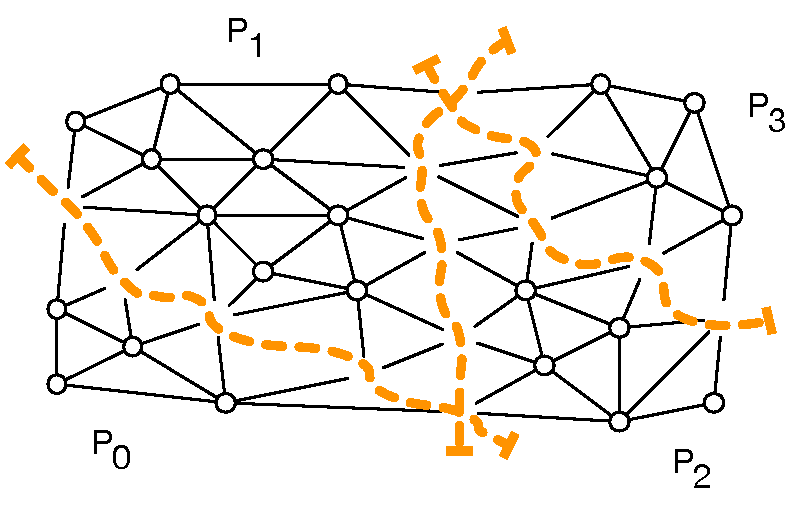
\includegraphics[scale=0.6]{sparsetiling/figures/partiotioned.pdf}
\caption{Partitioning of the seed loop. The vertices are illustrated to make the connectivity of the mesh clear, although they do not belong to any partition yet.}
\label{fig:st-initial-part-sm}
\end{figure}

As detailed in the next two sections, the inspection proceeds by populating $T_i$ with iterations from $L_1$ and $L_2$. The challenge of this task is guaranteeing that all data dependencies -- read after write, write after read, write after write -- are honored. The output of the inspector is eventually passed to the executor. The inspection carries sufficient information for computing sets of tiles in parallel. $T_i$ is always executed by a single thread/process and the execution is atomic; that is, it does not require communication with other threads/processes. When executing $T_i$, first all iterations from $L_0$ are executed, then all iterations from $L_1$ and finally those from $L_2$.

\subsection*{Inspection for Shared-Memory Parallelism}
Similarly to OP2, to achieve shared-memory parallelism we use coloring. Two tiles that are given the same color can be executed in parallel by different threads. Two tiles can have the same color if they are not connected, because this ensures the absence of race conditions through indirect memory accesses during parallel execution. In the example we can use three colors: red (R), green (G), and blue (B). $T_0$ and $T_3$ are not connected, so they are assigned the same color. The colored tiles are shown in Figure~\ref{fig:st-loop-0}. In the following, with the notation $T_i^c$ we indicate that the $i$-th tile has color $c$. 

\begin{figure}
\centering
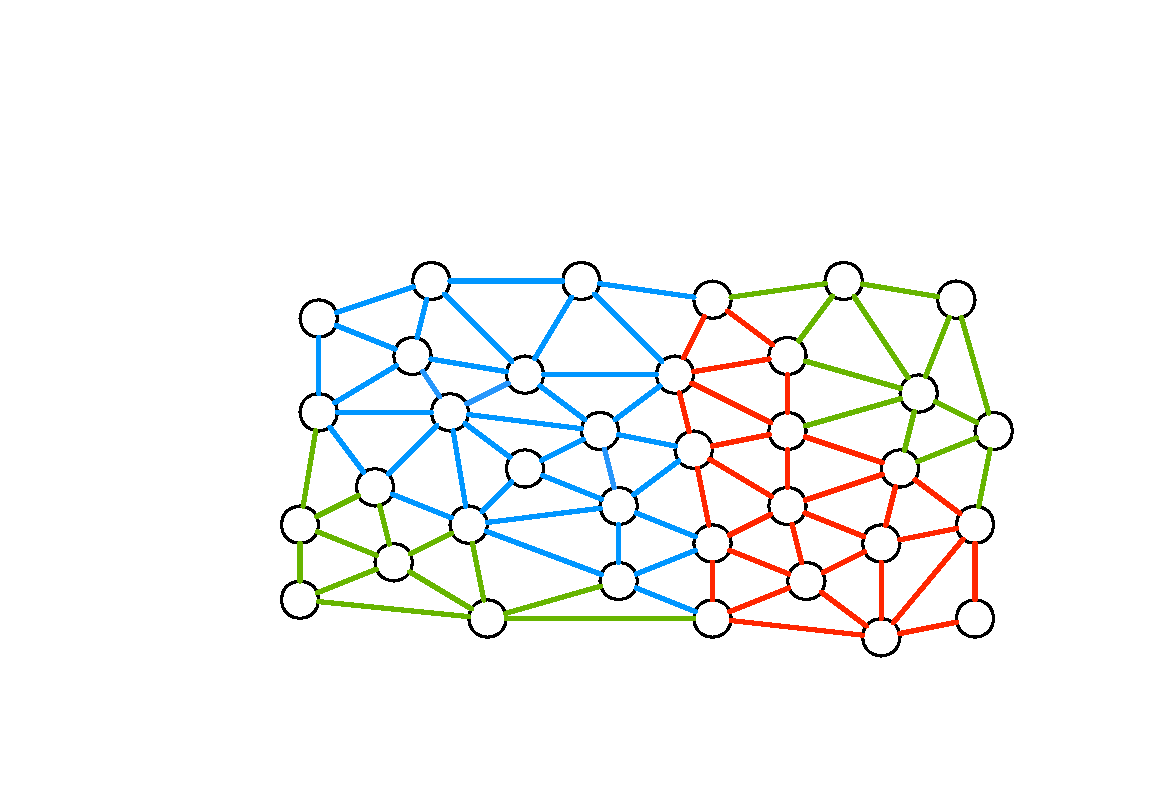
\includegraphics[scale=0.6]{sparsetiling/figures/loop_0.pdf}
\caption{A snapshot of the mesh after tiling $L_0$.}
\label{fig:st-loop-0}
\end{figure}

To populate $[T_0^G,\ T_1^B,\ T_2^R,\ T_3^G]$ with iterations from $L_1$ and $L_2$, we first have to establish a total ordering for the execution of partitions with different colors. Here, we assume the following order: green (G), blue (B), and red (R). This implies, for instance, that \textit{all iterations} assigned to $T_1^B$ must be executed \textit{before all iterations} assigned to $T_2^R$. By ``all iterations'' we mean the iterations from $L_0$ (determined by the seed partitioning) as well as the iterations that will later be assigned from tiling $L_1$ and $L_2$. We assign integer positive numbers to colors to reflect their ordering, where a smaller number means higher execution priority. We can assign, for example, 0 to green, 1 to blue, and 2 to red.

To schedule the iterations of $L_1$ to $[T_0^G,\ T_1^B,\ T_2^R,\ T_3^G]$, we need to compute a \textit{projection} for any write or local reduction performed by $L_0$. The projection required by $L_0$ is a function $\phi : V \rightarrow \mathbb{T}$ mapping the vertices in $V$ -- as indirectly incremented during the execution of $L_0$, see Listing~\ref{code:tiling-runningexample} -- to a tile $T_i^c \in \mathbb{T}$. Consider the vertex $v_0$ in Figure~\ref{fig:st-loop-0-proj}. $v_0$ has 7 incident edges, 2 of which belong to $T_0^G$, while the remaining 5 to $T_1^B$. Since we established that $G \prec B$, $v_0$ can only be read after $T_1^B$ has finished executing the iterations from $L_0$ (i.e., the 5 incident blue edges). We express this condition by setting $\phi(v_0) = T_1^B$. Observe that we can compute $\phi$ by iterating over $V$ and, for each vertex, applying the maximum function ($\operatorname{MAX}$) to the color of the adjacent edges. 

\begin{figure}
\centering
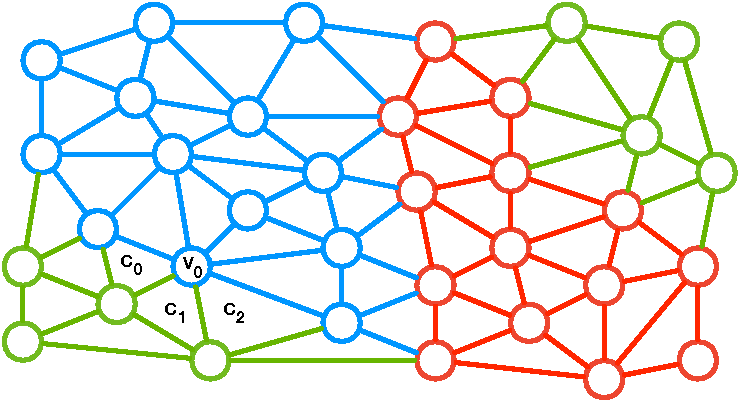
\includegraphics[scale=0.6]{sparsetiling/figures/loop_0_with_vertices.pdf}
\caption{The vertices are written by $L_0$, so a projection must be computed before tiling $L_1$. Here, the projection is represented by the colored vertices.}
\label{fig:st-loop-0-proj}
\end{figure}

\begin{figure}
\centering
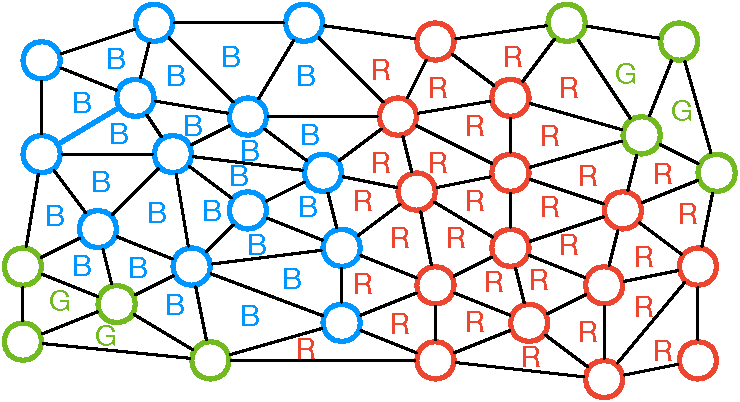
\includegraphics[scale=0.6]{sparsetiling/figures/loop_1.pdf}
\caption{A snapshot of the mesh after tiling $L_1$.}
\label{fig:st-loop-1}
\end{figure}

We now use $\phi$ to schedule $L_1$, a loop over cells, to the tiles. Consider again $v_0$ and the adjacent cells $[c_0,\ c_1,\ c_2]$ in Figure~\ref{fig:st-loop-0-proj}. These three cells have in common the fact that they are adjacent to both green and blue vertices. For $c_1$, and similarly for the other cells, we compute $\operatorname{MAX}(\phi(v_0),\ \phi(v_1),\ \phi(v_2)) = \operatorname{MAX}(B, G, G) = B = 1$. This establishes that $c_1$ must be assigned to $T_1^B$, because otherwise ($c_1$ assigned instead to $T_0^G$) a read to $v_0$ would occur before the last increment from $T_1^B$ took place. Indeed, we recall that the execution order, for correctness, must be ``all iterations from $[L_0, L_1, L_2]$ in the green tiles before all iterations from $[L_0, L_1, L_2]$ in the blue tiles''. The scheduling of $L_1$ to tiles is displayed in Figure~\ref{fig:st-loop-1}.

\begin{figure}[h]
\centering
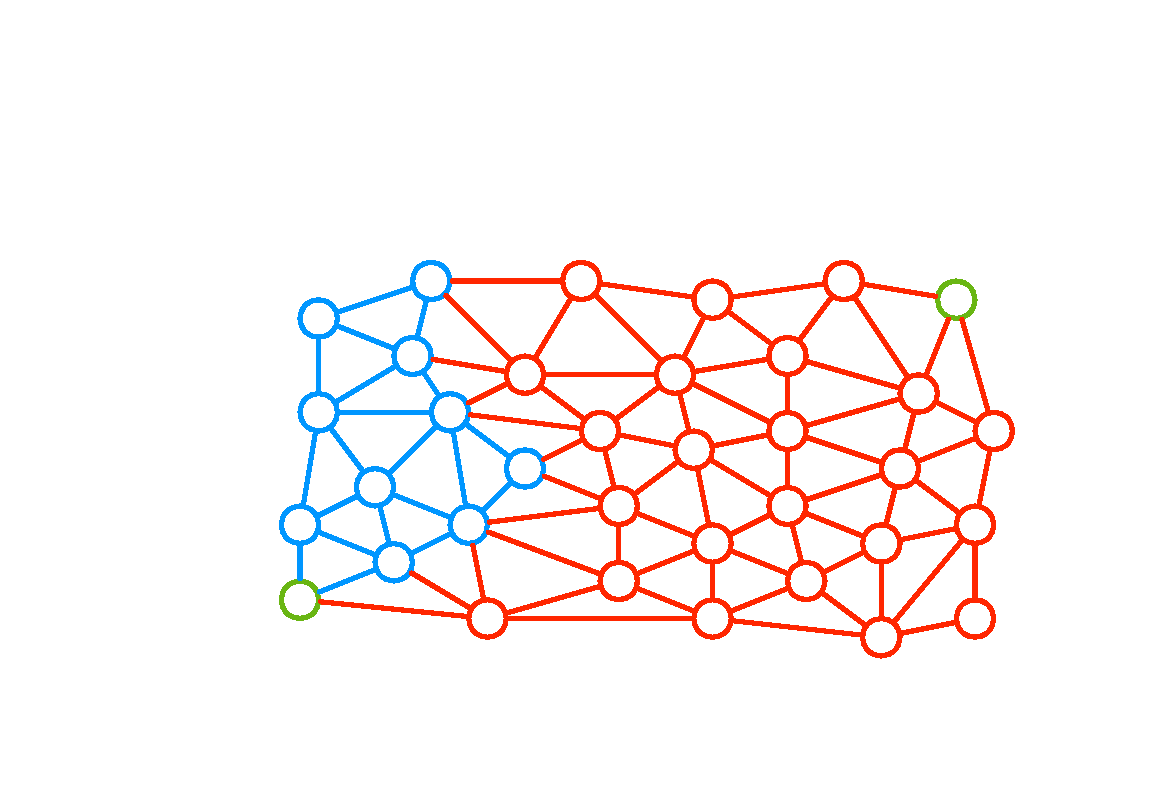
\includegraphics[scale=0.6]{sparsetiling/figures/loop_2.pdf}
\caption{A snapshot of the mesh after tiling $L_2$.}
\label{fig:st-loop-2}
\end{figure}

To schedule $L_2$ to $[T_0^G,\ T_1^B,\ T_2^R,\ T_3^G]$ we employ a similar process. Vertices are again written by $L_1$, so a new projection over $V$ will be necessary. Figure~\ref{fig:st-loop-2} shows the output of this last phase. 



\paragraph{Conflicting Colors}
It is worth noting how $T_2^R$ ``consumed'' the frontier elements of all other tiles every time a new loop was scheduled. Tiling a loop chain consisting of $k$ loops has the effect of expanding the frontier of a tile of at most $k$ vertices. With this in mind, we re-inspect the loop chain of the running example, although this time employing a different execution order -- blue (B), red (R), and green (G) -- and and a different seed partitioning. Figure~\ref{fig:st-conflicts} shows that, by applying the same procedure described in this section, $T_0^G$ and $T_3^G$ will eventually become adjacent. This violates the precondition that {\it tiles can be given the same color, and thus run in parallel, as long as they are not adjacent}. Race conditions during the execution of iterations belonging to $L_2$ are now possible. This problem will be solved in Section~\ref{sec:tiling:inspector}.

\begin{figure}[h]
\centering
\begin{subfigure}[b]{0.33\textwidth}
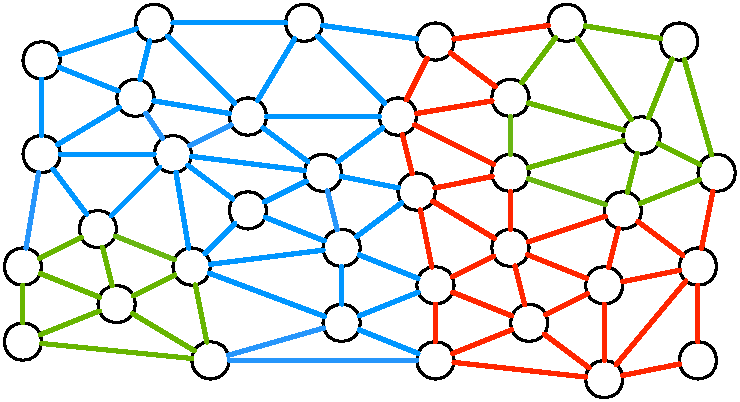
\includegraphics[width=\textwidth]{sparsetiling/figures/loop_0_conflicts.pdf}
\caption{After tiling $L_0$}
\label{fig:st-conflicts-a}
\end{subfigure}%
~ 
\begin{subfigure}[b]{0.33\textwidth}
\centering
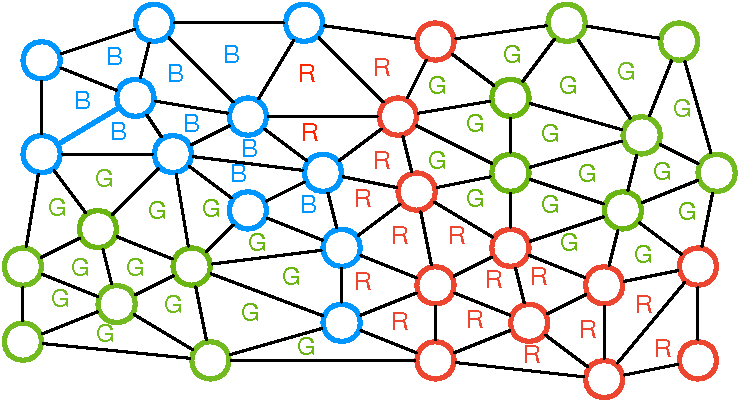
\includegraphics[width=\textwidth]{sparsetiling/figures/loop_1_conflicts.pdf}
\caption{After tiling $L_1$}
\label{fig:st-conflicts-b}
\end{subfigure}%
~
\begin{subfigure}[b]{0.34\textwidth}
\centering
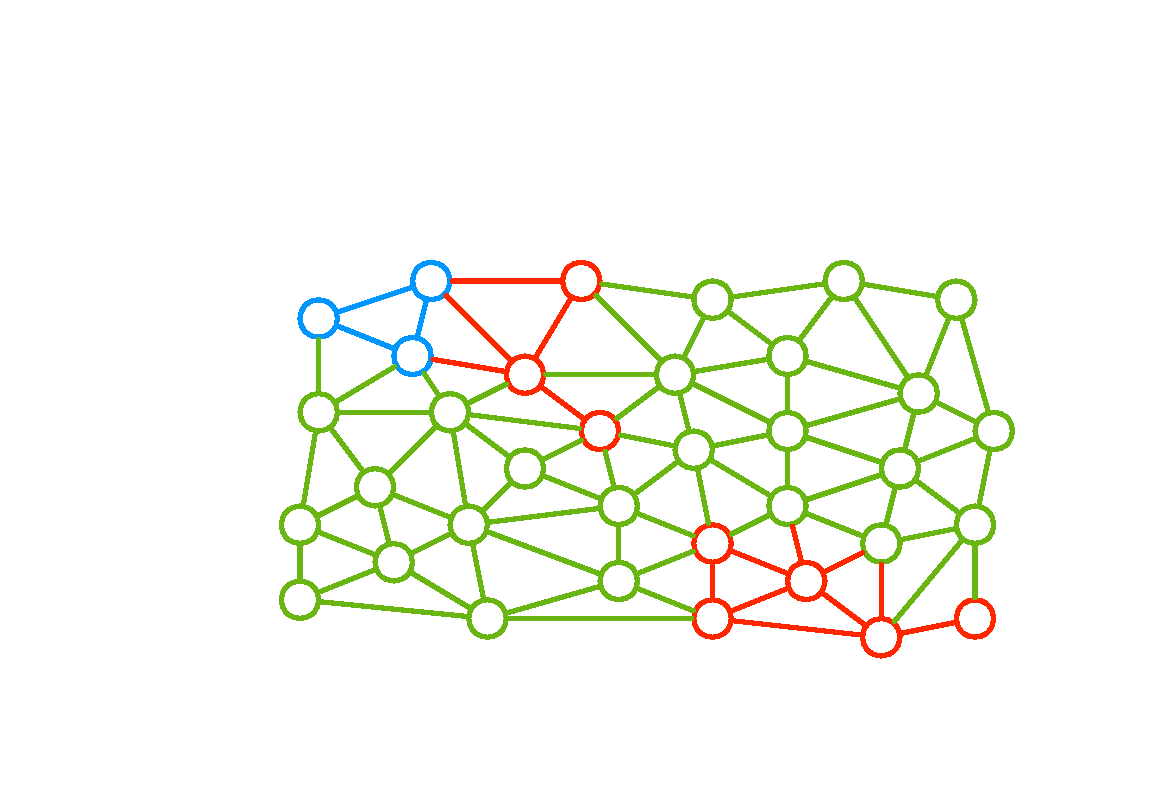
\includegraphics[width=\textwidth]{sparsetiling/figures/loop_2_conflicts.pdf}
\caption{After tiling $L_2$}
\label{fig:st-conflicts-c}
\end{subfigure}%

\caption{Tiling the program in Listing~\ref{code:tiling-runningexample} for shared-memory parallelism can lead to conflicts. Here, the two green tiles eventually become adjacent, creating race conditions.}
\label{fig:st-conflicts}
\end{figure}

\subsection*{Inspection for Distributed-Memory Parallelism}
If parallelism is achieved through message-passing, the mesh and its datasets are distributed to different processes. As in Listing~\ref{code:tiling-struct}, MPI calls now separate the execution of two consecutive loops in the chain. This means that our inspector/executor scheme will have to take extra care of data dependencies along the mesh partition boundaries.

From Section~\ref{sec:tiling:lc-unstruct} we know that all sets are logically split into three regions, \textit{core}, \textit{boundary}, and \textit{non-exec}. The boundary region includes all iterations that cannot be executed until the MPI communications have been accomplished. With this in mind, we take again $L_0$ as seed loop and make the following adjustments to the procedure that we have just described.
\begin{enumerate}
\item We take the core region of $L_0$ and partition it into tiles. Unless we aim for a mixed distributed/shared-memory parallelization scheme, there is no need to reassign the same color to unconnected tiles: now a single process executes sequentially its own tiles. We can assign colors increasingly, with $T_i$ given color $i$. As long as tiles with contiguous ID are also physically contiguous in the mesh, this assignment retains spatial locality when ``jumping'' from executing $T_i$ to $T_{i+1}$.
\item We replicate for the boundary region of $L_0$ what we just did for the core. By separating the core and boundary regions, we are preventing, by construction, a situation in which a tile crosses the two regions. Further, all tiles within the boundary region are given a color greater than then highest one in core. This constrains the execution order: no boundary tiles will be executed until all core tiles have been computed.
\item We map the whole non-exec region of $L_0$ to a single special tile, $T_{ne}$. This tile has the highest color and will actually never be executed. 
\end{enumerate}

From now on, the inspection proceeds as in the case of shared-memory parallelism. The application of the $\operatorname{MAX}$ function when scheduling $L_1$ and $L_2$ makes higher color tiles (i.e., those having lower priority) ``grow over'' lower color ones. 

Figure~\ref{fig:st-mpi-init} shows a distribution of the same mesh used in Figure~\ref{fig:st-initial-part-sm} to two processes, as well as a possible partitioning into tiles. It is worth observing that: (i) the whole boundary region is expanding over core, which is an essential requirement for correctness; (ii) the boundary region was sized to enable enough redundant computation, which in turn avoids synchronization.

\begin{figure}
\centering
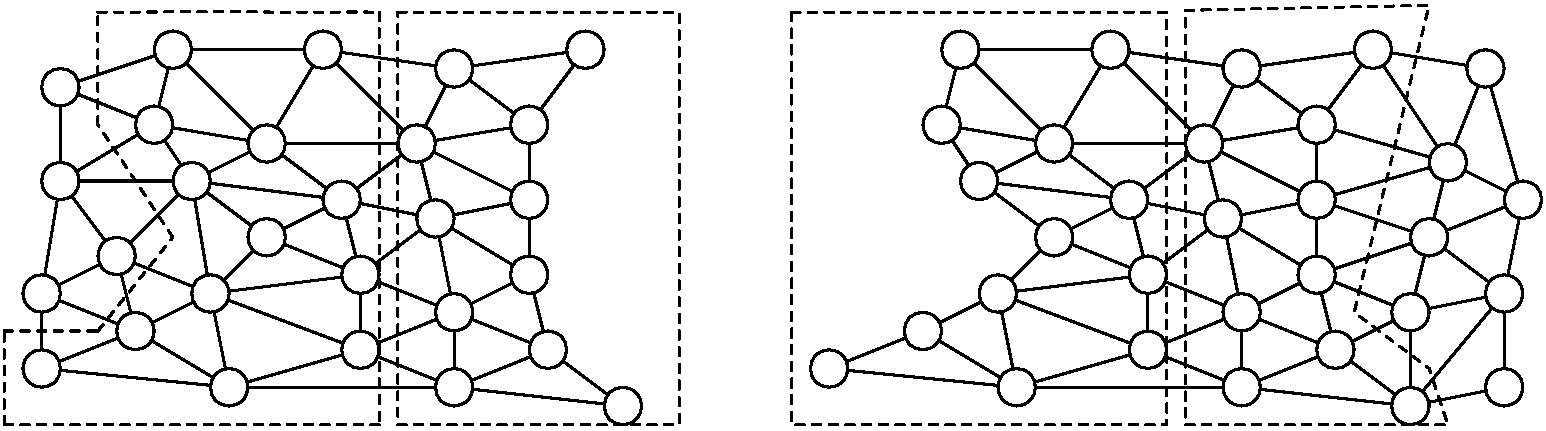
\includegraphics[width=\textwidth]{sparsetiling/figures/base_mesh_doppio.pdf}
\caption{Seed partitioning for distributed memory execution.}
\label{fig:st-mpi-init}
\end{figure}

We finally notice that:
\begin{description}
\item[Executor] On each process, the executor starts with triggering the MPI communications required for executing the boundary tiles. It proceeds to scheduling the core tiles, thus overlapping communication with computation. As all core tiles have finished executing and the MPI communications have terminated, the boundary tiles are computed.
\item[Correctness] This inspector/executor scheme relies on redundant computation along the boundaries of mesh partitions. The depth of the boundary region -- a parameter of the loop chain, as explained in Section~\ref{sec:tiling:lc-unstruct} -- grows proportionally with the number of loops that are fused. Roughly speaking, if the loop chain consists of $n$ loops, then the boundary region needs $n-1$ extra layers of elements. In Figure~\ref{fig:st-mpi-growth}, the elements in the green box belong to {\tt Process$_1$}, but they must also be accessed by {\tt Process$_0$} to update all elements in the yellow box correctly. The size of the green box (i.e., the amount of redundant computation) depends on $n$; that is, on how many loops one wants to fuse.
\item[Efficiency] The underlying hypothesis is that the increase in data locality achieved through sparse tiling will outweigh the cost of redundant computation. This is based on the consideration that the core region tends to be way larger than the boundary region. Moreover, not all iterations along the boundary region need be redundantly executed at every loop. The non-exec tile $T_{ne}$ is given the highest color, so it expands over the boundary region as new loops are tiled. This will create some dirty values (until the next round of MPI communications), which however will never be touched since $T_{ne}$ will not be scheduled for execution. 
\end{description}



%The main difference with respect to frameworks such as OP2 (see Section~\ref{sec:bkg:op2}) is that here, for reasons that will be more evident next, two regions, \textit{owned} and \textit{exec}, have been merged into a single one, \textit{boundary}. In essence, 


\section{Data Dependency Analysis for Loop Chains}

As with all loop optimizations that reschedule the iterations in a sequence of loops, any sparse tiling must satisfy the data dependencies. The loop chain abstraction, which we have described in Section~\ref{sec:tiling:lc}, provides enough information to construct an inspector which analyzes all of the dependencies in a computation and builds a legal sparse tiling. We recall that one of the main assumptions in a loop chain is that each loop is fully parallel or, equivalently, that there are no loop carried dependencies.

The descriptors in the loop chain abstraction enable a general derivation of the storage-related dependencies between loops in a loop chain. The storage related dependencies between loops can be described as either flow (read after write), anti (write after read), or output (write after write) dependencies. In the following, assume that loop $L_x$, having iteration space $S_x$, always comes before loop $L_y$, having iteration space $S_y$, in the loop chain. Let us identify a descriptor of a loop $L$ with $m_{S_i \rightarrow S_j}^{mode}$: this simply indicates that the loop $L_i$ has iteration space $S_i$ and uses a map $m$ to write/read/increment elements (respectively, $\texttt{mode} \in \lbrace w, r, i\rbrace$) in the space $S_j$.

The flow dependencies can then be enumerated by considering pairs of points ($\vec{i}$ and $\vec{j}$) in the iteration spaces of the two loops $L_x$ and $L_y$:
\[
	\{ \vec{i} \rightarrow \vec{j} \; | \; \vec{i} \in S_x \wedge \vec{j} \in S_y \wedge 
	m_{S_x\rightarrow S_z}^{w}(\vec{i}) \cap m_{S_y \rightarrow S_z}^{r}(\vec{j}) \ne \emptyset \}.
\]
Anti and output dependencies are defined in a similar way. The anti dependencies for all pairs of loops $L_x$ and $L_y$ are:
\[
	\{ \vec{i} \rightarrow \vec{j} \; | \; \vec{i} \in S_x \wedge \vec{j} \in S_y \wedge 
	m_{S_x\rightarrow S_z}^{r}(\vec{i}) \cap m_{S_y \rightarrow S_z}^{w}(\vec{j}) \ne \emptyset \}.
\]
While the output dependencies between loops $L_x$ and $L_y$ are:
\[
	\{ \vec{i} \rightarrow \vec{j} \; | \; \vec{i} \in S_x \wedge \vec{j} \in S_y \wedge 
	m_{S_x\rightarrow S_z}^{w}(\vec{i}) \cap m_{S_y \rightarrow S_z}^{w}(\vec{j}) \ne \emptyset \}.
\]
In essence, there is a storage-related data dependence between two iterations from different loops (and therefore between the tiles they are placed in) when one of those iterations writes to a data element and the other iteration reads from or writes to the same data element.

There are local reductions, or ``reduction dependencies'' between two or more iterations of the same loop when those iterations ``increment'' the same location(s); that is, when they read, modify with a commutative and associative operator, and write to the same location(s). The reduction dependencies in $L_x$ are:
\[
	\{ \vec{i} \rightarrow \vec{j} \; | \; \vec{i} \in S_x \wedge \vec{j} \in S_x \wedge m_{S_x\rightarrow S_z}^{i}(\vec{i}) \cap m_{S_x \rightarrow S_z}^{i}(\vec{j}) \ne \emptyset \}.
\]
The reduction dependencies between two iterations within the same loop indicates that those two iterations must be executed atomically with respect to each other.

As seen in the example in Section~\ref{sec:tiling:examples}, our inspector algorithm handles data dependencies, including those between non-adjacent loops, by tracking \textit{projections}. In the next section we explain how projections are constructed and used.

%In order to schedule $L$ to tiles, an up-to-date projection for each set $S$ accessed by $L$ must be available. For example, assume that $S$ is read by $L_k$ and is written by both $L_i$ and $L_j$. In the loop chain, the loops are in the order $L_i \prec ... \prec L_j \prec ... \prec L_k$. Let us denote by $\phi_S$ the projection for $S$. Each time that a loop accessing $S$ in write mode is inspected for scheduling, $\phi_S$ must be updated. When eventually scheduling $L_k$, therefore, an up-to-date snapshot of $\phi_S$ (i.e., the one produced right after tiling $L_j$) will be used to compute a legal tiling.

\clearpage


\section{Formalization}
\label{sec:tiling:algo}

\subsection{The Generalized Sparse Tiling Inspector}
\label{sec:tiling:inspector}

The pseudo-code for the generalized sparse tiling inspector is showed in Algorithm~\ref{algo:st-inspector}. Given a loop chain and an average tile size, the algorithm produces a schedule suitable for mixed distributed/shared-memory parallelism. In the following, we elaborate on the main steps of the algorithm. The notation used throughout the section is summarized in Table~\ref{table:st-summary-notation}.

\begin{table}[h]
\centering
\begin{tabulary}{1.0\columnwidth}{C|C}
\hline
Symbol & Meaning \\
\hline
$\mathbb{L}$ & The loop chain \\
$L_j$ & The $j$-th loop in $\mathbb{L}$ \\ 
$S_j$ & The iteration space of $L_j$ \\
$S_j^{c}$, $S_j^{b}$, $S_j^{ne}$ & The core, boundary, and non-exec regions of $S_j$ \\ 
$S$ & A generic set in $\mathbb{L}$ \\
$D$ & A descriptor of a loop \\
$r$, $w$, $i$ & Possible values for $D$.mode \\
$\mathbb{T}$ & The set of all tiles \\
$\mathbb{T}[i]$ & Accessing the $i$-th tile \\
%$T_i^{c}$, $T_i^{b}$ & the $i$-th tile over the core and boundary regions \\
$\phi_S$ & A projection $\phi_S : S \rightarrow \mathbb{T}$ \\
$\Phi$ & The set of all available projections \\
$\sigma_j$ & A tiling function $\sigma_j : S_j \rightarrow \mathbb{T}$ for $L_j$ \\
$ts$ & Average tile size \\
\hline
\end{tabulary}
\caption{Summary of the notation used throughout the section.}
\label{table:st-summary-notation}
\end{table}



\setcounter{algocf}{0}% Modify counter of algorithm
\begin{algorithm}[!t]

\SetKwData{SeedMap}{seed$\_$map}
\SetKwData{Conflicts}{conflicts}
\SetKwData{C}{C}
\SetKwFunction{AFC}{add$\_$fake$\_$connection}
\SetKwFunction{IFC}{has$\_$conflicts}
\SetKwFunction{CLM}{compute$\_$local$\_$maps}
\SetKwFunction{Color}{color}
\SetKwFunction{Partition}{partition}
\SetKwFunction{FindMap}{find$\_$map}
\SetKwFunction{Project}{project}
\SetKwFunction{Assign}{assign}
\SetKwFunction{Tile}{tile}

\kwInput{The loop chain $\mathbb{L} = [L_0,\ L_1,\ ...,\ L_{n-1}]$, a tile size $ts$}
\kwOutput{A set of tiles $\mathbb{T}$, populated with iterations from $\mathbb{L}$}
\nonl ~\\
\Comment{Initialization}
$seed \gets 0$\;
$\Phi \gets \emptyset$\;
$\C \gets \perp$\;
\nonl ~\\
\Comment{Creation of tiles}
$\sigma_{seed}$, $\mathbb{T} \gets$ \Partition{$S_{seed}$, $ts$}\;
\SeedMap $\gets$ \FindMap{$S_{seed}$, $\mathbb{L}$}\;
\Conflicts $\gets$ \False\;
\nonl ~\\
\Comment{Schedule loops to tiles}
\Do{\Conflicts}{
  \Color{$\mathbb{T}$, \SeedMap}\;
   \nonl ~\\
  \For{$j=1$ \KwTo $n-1$}{ \label{algo:st-tiling-loop}
    \Project{$L_{j-1}$, $\sigma_{j-1}$, $\Phi$, $C$}\;
    $\sigma_j \gets$ \Tile{$L_j$, $\Phi$}\;
    \Assign{$\sigma_j$, $\mathbb{T}$}\;
  }
  \nonl ~\\
  \If{\IFC{\C}}{
    \Conflicts $\gets$ \True\;
    \AFC{\SeedMap, \C}\;
  }
}
\nonl ~\\
\Comment{Inspection successful, create local maps and return}
\CLM{$\mathbb{T}$}\;
\Return{$\mathbb{T}$}
\caption{The inspection algorithm}
\label{algo:st-inspector}
\end{algorithm}





\paragraph{Choice of the seed loop}
The seed loop $L_{seed}$ is used to initialize the tiles. Theoretically, any loop in the chain can be chosen as seed. Supporting distributed-memory parallelism, however, is cumbersome if $L_{seed} \neq L_0$. This is because more general schemes for partitioning and coloring would be needed to ensure that no iterations in any $S_j^{b}$ are assigned to a core tile. A limitation of our inspector algorithm in the case of distributed-memory parallelism is that it must be $L_{seed} = L_0$. 

In the special case in which there is no need to distinguish between core and boundary tiles (because a program is executed on a single shared-memory system), $L_{seed}$ can be chosen arbitrarily. If we however pick $L_{seed}$ in the middle of the loop chain ($L_0 \prec ... \prec L_{seed} \prec ...$), a mechanism for constructing tiles in the reverse direction (``backwards''), from $L_{seed}$ towards $L_0$, is necessary. In~\cite{st-paper}, we propose two ``symmetric'' algorithms to solve this problem, \textit{forward tiling} and \textit{backward tiling}, with the latter using the $\operatorname{MIN}$ function in place of $\operatorname{MAX}$ when computing projections. For ease of exposition, and since in the fundamental case of distributed-memory parallelism we are imposing $L_{seed} = L_0$, we here neglect this distinction\footnote{The algorithm implemented in the library presented in Section~\ref{sec:tiling:impl-slope} supports backwards tiling for shared-memory parallelism.}. 

%\textit{Note: in real applications loops over ``subsets'' are possible; for instance, a loop over the exterior facets of the mesh. If one such loop is picked as seed, then the inspection is aborted.}



\paragraph{Tiles initialization}

\begin{table}[ht]
\centering
\begin{tabulary}{1.0\columnwidth}{P{2.7cm} | P{8.5cm}}
\hline
Field & Possible values \\
\hline
{\em region} & core, boundary, non-exec \\
{\em iterations lists} & one list of iterations $[T_i]_j$ for each $L_j \in \mathbb{L}$\\ 
{\em local maps} & one list of local maps for each $L_j \in \mathbb{L}$; one local map for each map used in $L_j$\\
{\em color} & an integer representing the execution priority \\ 
\hline
\end{tabulary}
\caption{The tile data structure.}
\label{table:st-tile-structure}
\end{table}

Let $ts$ be the user-specified average tile size. The algorithm starts with partitioning $S_{seed}^{c}$ into $m$ subsets $\lbrace P_0, P_1, ..., P_{m-1}\rbrace$ such that $|P_i| = ts$ (except possibly for $P_{m-1}$), $P_i \cap P_j = \emptyset$, and $\cup_{i = 0}^{m-1} P_i = S_{seed}^{c}$. Among all possible legal partitionings, we choose the one that splits $S_{seed}^c$ into blocks of $ts$ contiguous iterations, with $P_0 = \lbrace 0, ..., ts-1\rbrace$, $P_1 = \lbrace ts, ..., 2 ts - 1\rbrace$, and so on. We analogously partition $S_{seed}^{b}$ into $k$ subsets. We create $m+k+1$ tiles, one for each of these partitions and one extra tile for $S_{seed}^{ne}$. We therefore have $\mathbb{T} = \lbrace T_0^c, ..., T_{m-1}^c, T_m^{b}, ..., T_{m+k-1}^b, T_{m+k}^{ne} \rbrace$. 

A tile $T_i$ has four fields, as summarized in Table~\ref{table:st-tile-structure}. 

\begin{itemize}
\item The {\em region} is used by the executor to schedule tiles in a given order. This field is set right after the partitioning of $L_{seed}$, as a tile (by construction) exclusively belongs to $S_{seed}^c$, $S_{seed}^b$, or $S_{seed}^{ne}$.
\item The {\em iterations lists} contain the iterations in $\mathbb{L}$ that $T_i$ will have to execute. There is one {\em iterations list} $[T_i]_j$ for each $L_j \in \mathbb{L}$. At this stage of the inspection we have $[T_i]_{seed} = [T_i]_0 = P_i$, whereas still $[T_i]_j = \emptyset$ for $j=1,...,n$.
\item {\em Local maps} may be used for performance optimization by the executor in place of the global maps provided through the loop chain; this will be discussed in more detail in Section~\ref{sec:tiling:seigen}.
\item The {\em color} gives a tile a scheduling priority. If shared-memory parallelism is requested, adjacent tiles are given different colors (the adjacency relation is determined through the maps available in $\mathbb{L}$). Otherwise, colors are assigned in increasing order (i.e., $T_i$ is given color $i$). The boundary tiles are always given colors higher than that of core tiles; the non-exec tile has the highest color. The assignment of colors is carried by the function {\tt color} in Listing~\ref{algo:st-inspector}.
\end{itemize}



\paragraph{Populating tiles by tracking data dependencies}
To schedule a loop to tiles we use projections. A projection is a function $\phi_S : S \rightarrow \mathbb{T}$. Initially, the projections set $\Phi$ is empty. Each time a loop is tiled, $\Phi$ may be added some new projections or old projections may be updated. $\Phi$, and consequently the tiling functions for all loops in $\mathbb{L}$, are derived incrementally (within the loop at line~\ref{algo:st-tiling-loop} in Listing~\ref{algo:st-inspector}) starting from $\sigma_{seed} : S_{seed} \rightarrow \mathbb{T}$, the tiling function of $L_{seed}$. In the following, we discuss in detail how projections and tiling functions are constructed. 


\paragraph{Deriving a projection from a tiling function}

\begin{algorithm}[htp]
\SetKwData{Descriptors}{descriptors}
\SetKwData{Arity}{arity}
\SetKwData{AT}{$T_{last}$}
\SetKwData{MC}{max$\_$color}
\SetKwData{IM}{inverse$\_$map}
\SetKwData{Size}{size}
\SetKwData{Map}{map}
\SetKwData{Mode}{mode}
\SetKwData{D}{D}
\SetKwData{C}{C}
\SetKwData{Values}{values}
\SetKwData{Offset}{offset}
\SetKwData{Color}{color}
\SetKwFunction{MapInvert}{map$\_$invert}
\SetKwFunction{Update}{update}

\kwInput{A loop $L_j$, a tiling function $\sigma_j$, the projections set $\Phi$, the conflicts matrix $C$}
\KwResult{Update $\Phi$ and $C$}
\nonl ~\\
\ForEach{\D $\in$ $L_j$.\Descriptors}{
  \If{\D .\Mode $==$ r}{
    \Skip\;
  }
  \eIf{\D .\Map $==$ $\perp$}{
    $\Phi = \Phi \cup \sigma_{i}$\;
  }{
    \IM $\gets$ \MapInvert{\D .\Map}\;
    $S_t$, $S_j$, \Values, \Offset $\gets$ \IM\;
    $\phi_{S_t} \gets \perp$\; 
    \For{$e=0$ \KwTo $S_t$.\Size}{ \label{algo:st-projection-parallel}
      \For{$k= \Offset[e]$ \KwTo $\Offset[e+1]$}{
        \AT = $\mathbb{T}[\Values[k]]$\;
        \MC $\gets$ MAX($\phi_{S_{t}}[e]$.\Color, \AT .\Color)\;
        \If{\MC $\neq$ $\phi_{S_{t}}[e]$.\Color}{
          $\phi_{S_{t}}[e] \gets$ \AT\;
        }
      }
    }
    \Update{\C, $\mathbb{T}$, $\phi_{S_{t}}$}\;
    $\Phi = \Phi \cup \phi_{S_{t}}$\;
  }
}
\caption{Projection of a tiled loop}
\label{algo:st-projection}
\end{algorithm}

Algorithm~\ref{algo:st-projection} takes as input (the descriptors of) $L_{j}$ and its tiling function $\sigma_{j} :S_j \rightarrow \mathbb{T}$ to update $\Phi$. The algorithm also updates the conflicts matrix $C \in \mathbb{N}^{m \times m}$, which indicates whether two tiles having the same color will become adjacent once $L_{j+1}$ is tiled. 

A projection tells what tile a set element logically belongs to at a given point of the inspection. A new projection $\phi_{S}$ is needed if the elements of $S$ are written by a loop. Let us consider the non-trivial case in which writes or increments occur indirectly through a map $M : S_j \rightarrow S_t^0 \times S_t^1 \times ... \times S_t^{a-1}$. To compute $\phi_{S_{t}}$, we first determine the inverse map (an example is shown in Figure~\ref{fig:st-inverse-map}). Then, we iterate over all elements of $S_t$ and, for each $e \in S_t$, we determine the last tile that writes to $e$, say $T_{last}$. This is accomplished by applying the $\operatorname{MAX}$ function over the color of the tiles accessing $e$. We finally simply set $\phi_{S_{t}}[e] = T_{last}$. 


\begin{figure}[h]
\begin{CenteredBox}
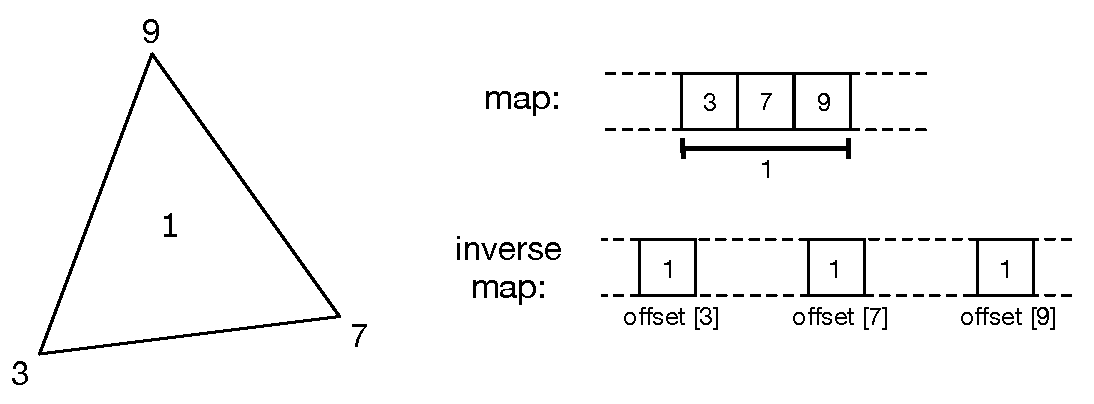
\includegraphics[scale=0.7]{sparsetiling/figures/inverse_map}
\end{CenteredBox}
\caption{Representation of an inverse map. The original map shows that the triangular cell $1$ is adjacent to three vertices, namely $3$, $7$, and $9$. The inverse map associates vertices to cells. Since the mesh is unstructured, different vertices can be incident to a different number of cells. The array {\tt offset} determines the distance between two consecutive vertices in the inverse map. For instance, all entries in the inverse map between {\tt offset[3]} and {\tt offset[4]} are cells incident to vertex $3$ (in the illustrated case, the first of these is cell $1$).}
\label{fig:st-inverse-map}
\end{figure}

% ($C[i,j] = 1$ implies that $T_i$ and $T_j$ have the same color and will become adjacent after tiling $L_{i-1}$).

\paragraph{Deriving a tiling function from the available projections}

\begin{algorithm}[htp]
\SetKwData{Descriptors}{descriptors}
\SetKwData{Arity}{arity}
\SetKwData{AT}{adjacent$\_$tile}
\SetKwData{MC}{max$\_$color}
\SetKwData{Size}{size}
\SetKwData{Map}{map}
\SetKwData{D}{D}
\SetKwData{Values}{values}
\SetKwData{Color}{color}

\kwInput{A loop $L_{j}$, the projections set $\Phi$}
\kwOutput{The tiling function $\sigma_{j}$}
\nonl ~\\
$\sigma_j \gets \perp$\;
\ForEach{\D $\in$ $L_j$.\Descriptors}{
  \eIf{\D .\Map $==$ $\perp$}{
    $\sigma_j \gets \Phi[S_j]$\;    
  }{
    \Arity $\gets$ D.\Map .\Arity\;
    $\phi_{S} \gets \Phi[\D.\Map.S_{j}]$\;
    \For{$e=0$ \KwTo $S_j$.\Size}{ \label{algo:st-tiling-parallel}
       $\sigma_j[e] \gets T_{\perp}$ \;
      \For{$k=0$ \KwTo \Arity}{
        \AT $\gets \phi_{S}[\D.\Map .\Values[e*\Arity + k]]$\;
        \MC $\gets$ MAX($\sigma_j[e]$.\Color, \AT .\Color)\;
        \If{\MC $\neq$ $\sigma_j[e]$.\Color}{
          $\sigma_j[e] \gets$ \AT\;
        }
      }
    }
  }
}
\Return{$\sigma_j$}
\caption{Building a tiling function}
\label{algo:st-tiling}
\end{algorithm}

Using $\Phi$, we compute $\sigma_j$ as described in Algorithm~\ref{algo:st-tiling}. The algorithm is similar to the projection of a tiled loop, with the main difference being that now we use $\Phi$ to schedule iterations correctly. Finally, $\sigma_j$ is inverted and the iterations are added to the corresponding iteration lists $[T_i]_j$, for all $T_i \in \mathbb{T}$. 


\paragraph{Detection of conflicts}
If $C$ indicates the presence of at least one conflict, say between $T_{i_1}$ and $T_{i_2}$, we add a ``fake connection'' between these two tiles and loop back to the coloring stage. $T_{i_1}$ and $T_{i_2}$ are now connected, so they will be assigned different colors. 
%Otherwise, a legal tiling has now been computed. 



\subsection{The Generalized Sparse Tiling Executor}

\begin{algorithm}[htpb]
\SetKwData{Color}{color}
\SetKwData{T}{T}
\SetKwFunction{SMC}{start$\_$MPI$\_$comm}
\SetKwFunction{EMC}{end$\_$MPI$\_$comm}
\SetKwFunction{GTBR}{group$\_$tiles$\_$by$\_$region}
\SetKwFunction{ET}{execute$\_$tile}

\kwInput{A set of tiles $\mathbb{T}$}
\KwResult{Execute the loop chain}
\nonl ~\\
$\mathbb{T}^{c}$, $\mathbb{T}^{b}$ $\gets$ \GTBR{$\mathbb{T}$}\;
\nonl ~\\
\SMC{}\;
\nonl ~\\
\ForEach{\Color}{
  \ForEach{$\T \in \mathbb{T}^{c}$ s.t. \T .\Color $==$ \Color}{ \label{algo:st-executor:parallel1}
    \ET{\T}\;
  }
}
\nonl ~\\
\EMC{}\;
\nonl ~\\
\ForEach{\Color}{
  \ForEach{$T \in \mathbb{T}^{b}$ s.t. \T .\Color $==$ \Color}{ \label{algo:st-executor:parallel2}
    \ET{\T}\;
  }
}
\caption{The executor algorithm}
\label{algo:st-executor}
\end{algorithm}


The sparse tiling executor is illustrated in Algorithm~\ref{algo:st-executor}. It consists of four main phases: (i) boundary exchange between processes through non-blocking MPI communications, (ii) execution of core tiles (in overlap with communication), (iii) waiting for the termination of all MPI communications, (iv) execution of boundary tiles.

As seen in the example in Section~\ref{sec:tiling:examples} and based on the explanation in Section~\ref{sec:tiling:inspector}, we know that the core tiles do not require any off-process information to execute as long as the boundary regions are (i) up-to-date and (ii) ``sufficiently deep''. If both conditions hold, the execution is semantically correct and it is safe to overlap computation of core tiles with the communication of boundary data. 


\paragraph{The depth of the boundary region}
In $\mathbb{L}$ we have $n$ loops. A tile ``crosses'' all of these loops and is executed atomically; that is, once it starts executing its iterations, it reaches the end without the need for synchronization with other processes. With this execution model, the boundary region must include a sufficient amount of off-process iterations for a correct computation of the tiles along the border with the core region. 

In the extreme case $n=1$ (i.e., no loop fusion), only a single ``strip'' of elements belonging to adjacent processes need be redundantly executed for overlapping computation and communication. As $n$ increases, more off-process data is required. In the example in Figure~\ref{fig:st-mpi-growth} we had $n=3$, so three ``strips'' of off-process elements were necessary for computing correctly the dataset associated with vertices when executing iterations belonging to $L_3$.

The {\em depth} is a parameter provided through the loop chain abstraction that informs the inspector about the extent of the boundary region. For correctness, we cannot fuse more than {\em depth} loops, so if $n$ is found to be larger than {\em depth}, we will need $\lceil \frac{n}{depth} \rceil$ different loop chains.

%For ease of explanation, this aspect has been neglected in the inspector algorithms described in the previous section. 

%Our inspector/executor strategy, therefore, works correctly as long as the loop chain has been ``dimensioned'' properly, with sufficient information in all $S^{b}$ regions 

%\paragraph{The execution of a tile}


\subsection{Computational Complexity of Inspection}


Let $N$ be the maximum size of a set in $\mathbb{L} = [L_0, L_1, ..., L_{n-1}]$ and let $M$ be the maximum number of sets accessed in a loop. If $a$ is the maximum arity of a map, then $K = a N$ is the maximum cost for iterating over a map. $K$ is also the worst-case cost for inverting a map. Let $p < 1$ be the probability that a conflict arises during inspection in the case of shared-memory parallelism; thus, the expected number of inspection rounds is $R = \frac{1}{1-p}$. Hence, the worst-case computational costs of the main inspection phases are as in Table~\ref{table:st-comp-cost}.

\begin{table}[h]
\centering
\begin{tabulary}{1.0\columnwidth}{P{2.7cm} | c | c}
\hline
Phase & Cost shared memory & Cost distributed memory \\
\hline
Partitioning & $N$ & $N$ \\
Coloring & $R K $ & $N$ \\ 
Projection & $R (n M N K^2) $ & $n M N K^2 $ \\ 
Tiling & $R (n M N K) $ & $n M N K $ \\
Local maps & $n M$ & $n M$\\
\hline
\end{tabulary}
\caption{Worst-case computational costs of the main inspection phases.}
\label{table:st-comp-cost}
\end{table}

%LOCAL MAPS: Finally, for each $T_i \in \mathbb{T}$, for each $L_j \in \mathbb{L}$, for each map used in $L_j$, create a local map. 

\section{Implementation}
\label{sec:tiling:automation}
The implementation of automated generalized sparse tiling is distributed over three software modules. 
\begin{description}
\item[Firedrake] The framework for the automated solution of PDEs through the finite element method (Section~\ref{sec:bkg:fenics-and-firedrake}).
\item[PyOP2] Firedrake produces numerical kernels to be applied over sets of mesh components. The parallel iteration over the mesh is handled by PyOP2 (Section~\ref{sec:bkg:op2}).
\item[SLOPE] A library for writing generalized inspector/executor schemes, with primary focus on sparse tiling. PyOP2 uses SLOPE for applying sparse tiling to loop chains.
\end{description}

There are several reasons that motivate this structuring.
\begin{description}
\item[Simplicity of analysis] The abstractions used in Firedrake and PyOP2 drastically simplify the analysis of input programs. For example, from the parallel loop construct in PyOP2 (Section~\ref{sec:bkg:op2}) we can derive all information we need to construct a loop chain.
\item[Flexibility] It is very intuitive to use sparse tiling in a Firedrake program. Once the regions of code to be sparse tiled are indicated, the inspector/executor schemes are automatically derived at the level of the run-time support. In the case of a PyOP2 program, the generation of inspector/executor schemes is only partly automated: the separation of a set into the core, boundary and non-exec regions for distributed-memory parallelism is here user's responsibility. An inspector-executor scheme can also be written from scratch, for instance in a plain C program. In this case, the loop chain must be provided explicitly through direct calls to the SLOPE library. 
\item[Realistic simulations] We aim to use generalized sparse tiling in real-world programs. The choice was then to use a framework, Firedrake, with a user base that could provide meaningful examples. The implementation effort is higher, but so is the potential scientific impact.
\end{description}

The interplay amongst Firedrake, PyOP2 and SLOPE is outlined in Figure~\ref{fig:st-implementation} and discussed in more detail in the following sections.

\begin{figure}[htpb]
\centering
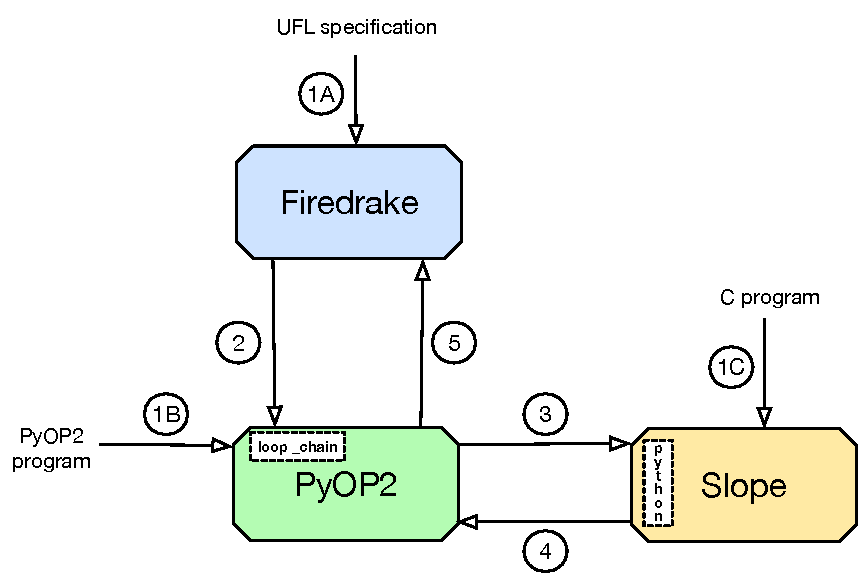
\includegraphics[scale=0.6]{sparsetiling/figures/firedrake-pyop2-slope.pdf}
\caption{Sparse tiling in the Firedrake-PyOP2-SLOPE framework. There are three ways of sparse tiling a loop chain: decorating UFL in a Firedrake program (1A), decorating a sequence of loops in a PyOP2 program (1B), writing both loop chain and inspector/executor codes explicitly in C through calls to SLOPE (1C). Both (1A) and (1B) use the {\em loop$\_$chain} interface (details in Section~\ref{sec:tiling:lcinterface}). The kernels generated within a {\em loop$\_$chain} are pre-processed in PyOP2 (2) and forwarded to SLOPE through its python interface (3). SLOPE has now access to the loop chain, so it can generate an inspector/executor scheme and return it to PyOP2 (4). The inspector is compiled and executed. The result, a schedule (i.e., the output of Algorithm~\ref{algo:st-inspector}), is cached and used as input to the executor. Each time the same {\em loop$\_$chain} is encountered in a Firedrake/PyOP2 program, the corresponding schedule is reused}.
\label{fig:st-implementation}
\end{figure}

\subsection{SLOPE: a Library for Sparse Tiling Irregular Computations}
\label{sec:tiling:impl-slope}
SLOPE is an open source software that provides an interface to build loop chains and to express inspector/executor schemes for sparse tiling\footnote{SLOPE is a contribution of this thesis and is available at \url{https://github.com/coneoproject/SLOPE}}. 

The loop chain abstraction implemented by SLOPE has been formalized in Section~\ref{sec:tiling:lc-unstruct}. In essence, a loop chain comprises some sets (including the separation into core, boundary, and non-exec regions), maps between sets, and a sequence of loops. Each loop has one or more descriptors specifying what and how different sets are accessed. The example in Listing~\ref{code:tiling-inspector} illustrates the interface exposed by SLOPE. 

SLOPE implements the algorithms in Section~\ref{sec:tiling:inspector}. Further, it provides additional features to estimate the effectiveness and to verify the correctness of sparse tiling:
\begin{description}
\item[VTK file generator] For each tiled loop, a file showing the mesh and the repartition into colored tiles is generated. The file is suitable for visualization in Paraview~\citep{paraview}.
\item[Inspection summary] The inspector returns useful information concerning the sparse tiling process, including: the number and the average size of tiles, the total number of colors used (which can partly explain the performance of a shared-memory parallelization), time spent in the critical inspection phases. 
\end{description}

In the case of shared-memory parallelism, the following sections of code are parallelized through OpenMP:
\begin{itemize}
\item The projection and tiling algorithms; in particular, the loop at line~\ref{algo:st-projection-parallel} of Algorithm~\ref{algo:st-projection} and the loop at line~\ref{algo:st-tiling-parallel} of Algorithm~\ref{algo:st-tiling}).
\item The execution of tiles having the same color; that is, the loops at lines~\ref{algo:st-executor:parallel1} and~\ref{algo:st-executor:parallel2} of Algorithm~\ref{algo:st-executor}.
\end{itemize}


\subsection{PyOP2: Lazy Evaluation and Interfaces}
\label{sec:tiling:lcinterface}
We focus on three relevant aspects of PyOP2: (i) the interface exposed for identifying loop chains; (ii) the lazy evaluation mechanism that allows building loop chains; (iii) the interaction with SLOPE for building and executing inspector/executor schemes.

To apply sparse tiling to a sequence of loops, PyOP2 provides the {\em loop$\_$chain} interface, exemplified in Listing~\ref{code:loop-chain-interface}. This interface is exposed to both users and Firedrake. In a Firedrake program, parallel loops may actually not appear at all in the source code, since they will automatically be generated from the UFL specification.

\begin{algorithm}[htpb]
\scriptsize\ttfamily
\SetAlgorithmName{LISTING}{}
\KwSty{with} {\em loop$\_$chain} (name, tile$\_$size, mode, ...):\\
~~~~Any Python code here, including UFL of PyOP2 loops\\
\caption{The {\em loop$\_$chain} interface in PyOP2. The {\tt name} is compulsory as it uniquely identify a loop chain, while all other parameters are optional. The optional parameters are useful for performance evaluation (e.g., logging) and performance tuning. The {\tt tile$\_$size} specifies the initial average size for the seed partitions. The {\tt mode} allows users to specify how to break a loop chain into smaller loop chains, thus simplifying experimentation with a whole set of sparse tiling schemes.}
\label{code:loop-chain-interface}
\end{algorithm}

PyOP2 exploits lazy evaluation of parallel loops to generate an inspector/executor scheme. The parallel loops encountered during the program execution -- or, analogously, those generated through Firedrake -- are not scheduled immediately; rather, they are pushed into a queue. The sequence of parallel loops in the queue is called {\em trace}. If a dataset $f$ needs be read, for example because a user wants to inspect its values or a global linear algebra operation needs be performed, the trace is traversed -- from the most recent parallel loop to the oldest one -- and a new sub-trace produced. The sub-trace includes all parallel loops that must be executed for correctly evaluating $f$. The sub-trace can then be executed or further pre-processed.

All loops in a trace that were created within a {\em loop$\_$chain} scope are sparse tiling candidates. In detail, the interaction between PyOP2 and SLOPE is as follows:
\begin{enumerate}
\item The example in Listing~\ref{code:loop-chain-interface} shows that a {\em loop$\_$chain} defines a new scope. As this scope is entered, a stamp $s_1$ of the trace is generated. This happens ``behind the scenes'', because the {\em loop$\_$chain} is a Python context manager, which can execute pre-specified routines prior and after the execution of the body. As the {\em loop$\_$chain}'s scope is exited, a new stamp $s_2$ of the trace is computed. All parallel loops generated between $s_1$ and $s_2$ are placed into a list for pre-processing.
\item The pre-processing consists of two steps: (i) ``simple'' fusion -- consecutive parallel loops iterating over the same iteration space that do not present indirect data dependencies are merged; (ii) generation of a loop chain representation for SLOPE, discussed next.
\item PyOP2 inspects the sequence of loops and translates all relevant data structures (sets, maps, loops) into a format suitable for the SLOPE's Python interface. C code implementing an inspector for the loops in the {\em loop$\_$chain} is returned by SLOPE. PyOP2 compiles and executes this code, which results in an {\em inspection} for the loop chain.
\item A ``software cache'' mapping {\em loop$\_$chain}s to {\em inspection}s is used. This whole process needs therefore be executed only once for a given {\em loop$\_$chain}. 
\item The executor is built in an analogous way to the inspector.
\end{enumerate}


\subsection{Firedrake/DMPlex: the S-depth mechanism for MPI}
\label{sec:tiling:impl-firedrake}
Firedrake uses DMPlex~\citep{dmplex-cite} to handle meshes. DMPlex is responsible for partitioning, distributing over multiple processes, and locally reordering a mesh. The MPI parallelization is therefore managed through Firedrake/DMPlex.

During the start-up phase, each MPI process receives a contiguous partition of the original mesh from DMPlex. The required PyOP2 sets, which can represent either topological components (e.g., cells, vertices) or function spaces, are created. As explained in Section~\ref{sec:bkg:op2}, these sets distinguish between multiple regions: core, owned, exec, and non-exec. Firedrake initializes the four regions exploiting the information provided by DMPlex. 

To support the loop chain abstraction, Firedrake must be able to allocate arbitrarily deep halo regions. Both Firedrake and DMPlex have been extended to support this feature\footnote{The implementation was mostly carried out by Michael Lange.}. A parameter called {\em S-depth} (the name has historical origins, see for instance~\cite{s-depth-paper}) regulates the extent of the halo regions. A value $S{-}depth=n$ indicates the presence of $n$ strips of off-process data elements in each set. The default value is $S{-}depth=1$, which enables computation-communication overlap when executing a single loop at the price of a small amount of redundant computation along partition boundaries. This is the default execution model in Firedrake.


\section{Performance Evaluation}
The experimentation was characterized by two phases:

\begin{enumerate}
\item Generalized sparse tiling was initially applied to two benchmarks: a sparse Jacobi kernel and a proxy unstructured mesh application, originally developed as a demo for the OP2 framework. This was especially useful to identify strengths and limitations of the technique.
\item Then, it was used in an application developed in Firedrake, Seigen, an Elastic Wave Equation Solver for Seismological Problems\footnote{Seigen has been developed by Christian Jacobs.}. The aim of this phase was to evaluate the performance improvements in a realistic simulation.
\end{enumerate}

%note: tile size independent of mesh size !!!! but actually dependent on the application...!


\subsection{Benchmarks}
In this section, our objective is to explore the impact of generalized sparse tiling on performance, to characterize the circumstances where the approach is profitable, to identify the major limitations to a widespread adoption of the technique, and to justify some of the design choices made in the previous sections.

All benchmarks are written in C. The sparse tiled implementations only support shared-memory parallelism via OpenMP. A previous version of the inspector algorithms presented in this chapter, described in~\cite{st-paper}, was used. As detailed next, one of the major drawbacks of this older inspector was its cost, which grew very rapidly with the number of loops in the chain and the number of distinct datasets accessed. 

In all the experiments presented in this section, the optimal tile size (i.e. the one leading to the best execution time) was determined empirically, for each combination of architecture and application. 

\subsubsection{Sparse Jacobi}

\begin{table}[t]
\centering
\begin{tabulary}{1.0\columnwidth}{c | c | c}
\hline
Matrix name & Execution time reduction & Speed-up  \\
\hline
{\em ldoor} & 40.34 & 12.11 \\
{\em pwtk} & 38.42 & 11.98 \\
{\em thermal2} & 25.78 & 11.08 \\
{\em xenon2} & 20.15 & 9.53 \\
{\em audikw$\_$1} & 13.42 & 8.70 \\
{\em nd24k} & -151.72 & 3.06 \\
\hline
\end{tabulary}
\caption{Execution time reductions over the original implementation (in percentage) and speed-ups over the single-threaded tiled implementation for the sparse Jacobi solver with 15 threads.}
\label{table:st-jacobi}
\end{table}

The first experiment was the full sparse tiling of a Jacobi sparse matrix solver\footnote{This section is partly extracted from~\cite{st-paper}, and the results were obtained from experiments conducted by Christopher D. Krieger, Catherine Olschanowsky, and Michelle Mills Strout}. Given a sparse matrix $A$, and a vector $\vec{f}$, related by $A\vec{u}=\vec{f}$, each iteration of the sparse Jacobi method produces an approximation to the unknown vector $\vec{u}$. In our experiments, the Jacobi convergence iteration loop is unrolled by a factor of two and the resulting two loops are chained together (1000 iterations of the loop chain was executed). Using a ping-pong strategy, each loop reads from one copy of the $\vec{u}$ vector and writes to the other copy. This experiment was run on an Intel Westmere (dual-socket 8-core Intel Xeon E7-4830 2.13 GHz, 24MB shared L3 cache per socket). The code was compiled using {\tt gcc-4.7.0} with options {\tt -O3 -fopenmp}.

The Jacobi recurrence equation includes a sparse matrix vector multiplication and is representative of a broad class of sparse linear algebra applications. It is also an effective test-bed because different data dependency patterns can be examined simply by using different input matrices. In these experiments, a set of 6 input matrices, drawn from the University of Florida Sparse Matrix Collection~\citep{ST-MatrixMarket}, was used. The matrices were selected so that they would vary in overall data footprint, from 45 MB to 892 MB, and in percentage of non-zeros, from very sparse at 0.0006\% to much more dense at 0.5539\% non-zeros. % values.

Table~\ref{table:st-jacobi} compares the performance of the tiled Jacobi solver to that of a simple blocked version. Both codes use OpenMP \texttt{parallel for} directives to achieve parallelism. The execution time reduction varied from 13$\%$ to 47$\%$ with the exception of the {\em nd24k} matrix, which showed as much as a 1.52x slowdown when sparse tiled. This matrix is highly connected, thus limiting the number of tiles that can be scheduled in parallel. The greater parallelism available under a blocked approach provides more benefit in this case than the performance improvements due to improved locality from full sparse tiling. Overall, speed-ups of between 8 and 12 times over the single-threaded tiled implementation were observed when using 15 threads; a clear outlier is again the {\em nd24k} matrix that did not scale past 3.2 times the single thread performance.

%and typically decreased as threads were added. We believe that this reduction is also related to the parallelism available in the task graph and are investigating methods to mitigate its impact.

The values in Table~\ref{table:st-jacobi} do not include the inspection time necessary to full sparse tile the loop chain. To break even when this cost is considered, the inspector time must be amortized over between 1000 and 3000 iterations of the executor, depending on the specific matrix being solved. We will further elaborate on this aspect in Section~\ref{sec:tiling:bench:conc}.



\subsubsection{Airfoil}


\begin{table}[t]
\centering
\begin{tabulary}{1.0\columnwidth}{c | c | c}
\hline
Implementation & Execution time & Speed-up \\
\hline
Westmere {\em omp} & 36.87 & 6.43\\
Westmere {\em mpi} & 31.0 & 7.66 \\
Westmere {\em tiled} & 26.49 & 8.96 \\
\hline \hline
Sandy Bridge {\em omp} & 30.01 & 6.65 \\
Sandy Bridge {\em mpi} & 24.42 & 8.17 \\
Sandy Bridge {\em tiled} & 20.63 & 9.67 \\
\hline
\end{tabulary}
\caption{Execution time (in seconds) and speed-ups over the slowest single-threaded implementation for the Airfoil benchmark. The values are obtained from simulations with fully-loaded machines (16 and 24 threads/processes on the Sandy Bridge and the Westmere architectures, respectively).}
\label{table:st-airfoil}
\end{table}

Airfoil is a representative unstructured mesh application~\citep{AIRFOIL}. Three implementations of Airfoil, {\em omp}, {\em mpi} and {\em tiled}, were compared on two shared-memory machines, an Intel Westmere (dual-socket 6-core Intel Xeon X5650 2.66 GHz, 12MB of shared L3 cache per socket) and an Intel Sandy Bridge (dual-socket 8-core Intel Xeon E5-2680 2.00Ghz, 20MB of shared L3 cache per socket). The code was compiled using the Intel \texttt{icc 2013} compiler with optimizations enabled (\texttt{-O3}, \texttt{-xSSE4.2/-xAVX}).

The Airfoil code consists of a main time loop with 2000 iterations. This loop contains a sequence of four parallel loops that carry out the computation. In this sequence, the first two loops, called $adt$-$calc$ and $res$-$calc$, constitute the bulk of the computation. $Adt$-$calc$ iterates over cells, reads from adjacent vertices and write to a local dataset, whereas $res$-$calc$ iterates over edges and exploits indirect mappings to vertices and cells for incrementing indirect datasets associated to cells. These loops share datasets associated with cells and vertices. Datasets are composed of doubles.
%-precision floating-point values.

In the {\em omp} and {\em mpi} implementations of Airfoil, the OpenMP and the MPI back-ends of OP2, were used. The effectiveness of these parallelization schemes has been demonstrated in~\cite{op2-main}. The {\em tiled} implementation uses an early version of the SLOPE library (the differences with the inspector algorithms shown in Section~\ref{sec:tiling:inspector} are discussed later) for tiling a loop chain. We manually unrolled the time loop by a factor of two to be able to tile over 6 loops in total. 

%The OP2 gFST library uses $METIS$~\cite{METIS} for computing a seed partitioning of the mesh vertices.

Table~\ref{table:st-airfoil} shows the scalability and runtime reduction achieved by sparse tiling the loop chain on the Westmere and Sandy Bridge architectures. The input unstructured mesh was composed of 1.5 million edges. It is worth noticing that both the {\em omp} and {\em tiled} versions suffer from the well-known NUMA effect as threads are always equally spread across the two sockets. Nevertheless, compared to {\em mpi}, the {\em tiled} version exhibits a peak runtime reduction of 15\% on the Westmere and of 16\% on the Sandy Bridge. 

Results shown for {\em tiled} do not include, however, the inspector overhead. By also including it, the aforementioned improvements over {\em mpi} reduce to roughly 10\% on both platforms. Similarly to the sparse Jacobi solver, the slow-downs when including the inspection overhead are significant.


\subsubsection{Observations}
\label{sec:tiling:bench:conc}
One of the most important outcomes of this first set of experiments concerns the inspection cost, which we found to significantly impact the overall execution time. To effectively support real applications like Seigen, typically characterized by a number of parallel loops larger than that of these benchmarks, we had to rework the original inspector algorithms into the versions described in Section~\ref{sec:tiling:inspector}. The most notable differences are: (i) data dependency analysis abstracted to the level of sets, rather than datasets; (ii) optimistic coloring with backtracking in case of conflicts; (iii) fully parallel projection and tiling phases, through the use of inverse maps. 

A second observation is about the importance of automation. Writing the inspector as a sequence of calls to SLOPE is relatively simple, although tedious and error-prone. Much more complicated is integrating the executor, because this essentially means rewriting entire sequences of loops -- a severe limitation when using SLOPE in plain C (perhaps legacy) code. These considerations on the implementation complexity led to the multilayer framework detailed in Section~\ref{sec:tiling:automation} for automating the generation of inspector/executor schemes. 

The Airfoil experiments highlighted that shared-memory parallelism over multi-socket architectures is considerably affected by the NUMA issue. The difference in execution time between the OP2 OpenMP and MPI versions is indeed remarkable. As discussed in~\cite{hydra-op2}, the irregular nature of the computation makes it hard to find systematic solutions to the NUMA problem when relying on OpenMP. The MPI and the hybrid OpenMP/MPI execution models are simply better candidates for unstructured mesh computations. The sparse tiled implementation, which in these experiments is also purely based on OpenMP, suffers from the NUMA issue as well, although it manages to outperform the OP2 MPI version thanks to the relieved memory pressure. We wondered, however, what the gain would be if we managed to integrate MPI with sparse tiling. This led to the definition of more general loop chain abstraction (Section~\ref{sec:tiling:lc-unstruct}) and inspector algorithms (Section~\ref{sec:tiling:inspector}), for supporting MPI-based executors.

\subsection{Seigen: an Elastic Wave Equation Solver for Seismological Problems}
\label{sec:tiling:seigen}
...

\section{Conclusions and Future Work}
%1) ... aggressive mode of firedrake, automatic tiling ?
%2) ...larger chunks communciated in the whole app if sdepth greater than 1, even outside of loop chain
